\chapter{Simuleren van gedrag op basis van een sequentiediagram}\label{sec:gedrag}
Een ander populair type van UML-diagram is het sequentiediagram\cite{RumbaughJames2005Tuml}. Waar klassediagrammen de informatie bevat in klasses en de verbanden tussen klasses benoemen, beschrijven sequentiediagrammen het gedrag van methodes gedefinieerd voor deze klasses. In deze diagrammen communiceren instanties van klasses via berichten. Doorgaans zijn deze berichten een oproep van een methode, of een toekenning aan een variabele intern aan het diagram of een instantiatie van een nieuwe instantie. De berichten zijn genummerd volgens een bepaalde volgorde en samen modelleren ze het gedrag van een stuk van de software.

Dit hoofdstuk beschrijft hoe we vocabularia en logische theorie\"en gegenereerd volgens de regels beschreven in sectie \ref{sec:cd-rep-cons} kunnen uitbreiden om het gedrag voorgesteld in een sequentiediagram te modelleren.

Sectie \ref{sec:sd-components} beschrijft de verscheidene componenten van een sequentiediagram en hun betekenis. Sectie \ref{sec:sd-ltc} benoemt het mechanisme dat we gebruiken om deze componenten voor te stellen in FO($\cdot$) en waarom we dat mechanisme gebruiken. Secties \ref{sec:sd-voc} tot en met \ref{sec:interaction} bouwen de regels voor onze voorstelling op. Ten slotte lijst sectie \ref{sec:beperkingen} de beperkingen op geldige sequentiediagrammen in de context van onze voorstelling op.

\section{Componenten van een sequentiediagram}\label{sec:sd-components}

Deze sectie beschrijft welke componenten we beschouwen in deze masterproef. We beperken in bepaalde aspecten de mogelijkheden voor de ontwerptaal beschikbaar voor sequentiediagrammen. Dit doen we om bij inferentie op de theorie\"en resulterend uit het vertaalproces beschreven in dit hoofdstuk de rekentijd en het geheugengebruik binnen de perken te houden.

Figuur \ref{fig:seq-diagram-game} geeft een voorbeeld van een sequentiediagram gebaseerd op het klassediagram voorgesteld in figuur \ref{fig:diagram-voorbeeld}. Het modelleert het gedrag van de methode \textit{attackWith(Character, Weapon)} gedefinieerd voor de klasse \textit{Character}.

Een instantie wordt voorgesteld door een kader met daarin tekst volgens het patroon \textit{instantienaam : klassenaam}. Dit wil zeggen dat bijvoorbeeld \textit{attacker} een instantie is van de klasse \textit{Character}. Vanuit elk kader vertrekt ook een streepjeslijn: De \textbf{levenslijn}. Deze levenslijn kan ingevuld worden door gekleurde balken, welke de duur van een oproep van een methode aan een instantie voorstellen.
Verder zijn er ook kaders die berichten omsluiten. Deze kaders duiden \textbf{gecombineerde fragmenten} aan, en deze tekst beschouwt twee soorten:

\begin{enumerate}
	\item Het \textbf{altfragment}: Deze soort duidt een \textit{if-else}-constructie aan. Het bestaat uit twee delen, namelijk het \textit{if}-deel en het \textit{else}-deel, en er staat aangeduid onder welke voorwaarden welk deel wordt uitgevoerd. Figuur \ref{fig:seq-diagram-game} bevat een voorbeeld van een altfragment.
	\item Het \textbf{lusfragment}: Deze soort duidt een lusconstructie aan. Er staat aangeduid onder welke voorwaarden er een iteratie wordt uitgevoerd. Deze voorwaarde wordt gecontroleerd zowel v\'o\'or de eerste keer dat er mogelijks een iteratie wordt uitgevoerd als elke keer dat een iteratie ten einde komt. Indien de voorwaarde niet geldt, wordt de lus overgeslagen. Figuur \ref{fig:seq-diagram-frag-ex} bevat een voorbeeld van een diagram met lusfragmenten.
\end{enumerate}

Berichten worden voorgesteld door pijlhoofden aan ofwel een ononderbroken lijn ofwel een streepjeslijn. Ze kunnen verscheidene betekenissen hebben afhankelijk van de context.

Er zijn berichten die een variabele defini\"eren en er een waarde aan toekennen. Die waarde kan direct berekend worden, zoals in instructie 12 in figuur \ref{fig:seq-diagram-game}. De waarde kan een directe waarde zijn zoals 3 of ``foo'', een variabele, of een bewerking op directe waarden of variabelen van primitieve types. Als de instructie een bewerking op waarden van een primitief type is, moeten de gebruikte waardes allemaal van hetzelfde type zijn en moet het type een geldig invoertype voor de bewerking zijn, anders is het sequentiediagram ongeldig. De toegekende waarde kan ook het resultaat zijn van een methodeoproep, zoals in instructie 3 in dezelfde figuur. Als de methode die wordt opgeroepen een methode is gedefinieerd voor een klasse door het klassediagram, wordt de waarde eerst berekend in een uitvoering van het bijhorend sequentiediagram v\'o\'or het wordt toegekend aan de variabele.

Een numerieke variabele kan een waarde krijgen door middel van de functies \textit{chooseEx(lowerBound, upperBound)} en \textit{chooseIn(lowerBound, upperBound)}. Bij uitvoering van die functies geeft de gebruiker een getal $n$ op. Bij \textit{chooseEx} geldt dat $n \geq lowerBound$ en $n < upperBound$ en bij \textit{chooseIn} geldt dat $n \geq lowerBound$ en $n \leq upperBound$.

Een variabele kan ook gedefinieerd worden door een paar van methodeoproep en terugkeerbericht. Instructies 6 en 7 in figuur \ref{fig:seq-diagram-game} zijn daar een voorbeeld van. Instructie 6 is een methodeoproep. Instructie 7 definieert impliciet de variabele \textit{defenceVal} en kent de waarde berekend in de oproep eraan toe.

Een oproep van een methode die \textit{void} als resultaattype heeft mag niet gepaard gaan met een definitie van of toekenning aan een variabele.

Methodeoproepen zijn enkel geldig als de methode die wordt opgeroepen gedefinieerd is voor de klasse waar de ontvanger van het bericht een instantie van is. Als een methode gedefinieerd voor een klasse in het klassediagram wordt opgeroepen, wordt verwacht dat voor elke parameter een geldige waarde van het juiste type wordt opgegeven, hetzij een directe waarde, hetzij een variabele. Indien het verkeerde aantal argumenten wordt opgegeven, is het gedrag van de oproep niet gedefinieerd. Indien een waarde van een fout type wordt opgegeven, is het sequentiediagram niet geldig.

Attributen en associaties defini\"eren voor klasses impliciet enkele methodes. 

We beschouwen enkel attributen met een multipliciteit van $1..1$. Daarvoor defini\"eren we methodes volgens de patronen \textit{getAttribuutnaam()} en \textit{setAttribuutnaam()}. Voor \textit{value} in de klasse \textit{Statistic} in figuur \ref{fig:diagram-voorbeeld} krijgen we \textit{getValue()} en \textit{setValue(int)}. \textit{getValue()} haalt de waarde van \textit{value} op en \textit{setValue(int)} zorgt ervoor dat de waarde van \textit{value} gelijk is aan de gegeven waarde in de volgende tijdstap.

Wat betreft associaties beschouwen we enkel binaire associaties. Ze defini\"eren de volgende soorten van methodes:

\begin{itemize}
	\item De multipliciteit is $1..1$: We defini\"eren een methode volgens het patroom \textit{getKlassenaam()}. De klasse \textit{Character} in figuur \ref{fig:diagram-voorbeeld} krijgt dus de methode \textit{getInventory()} dat de gerelateerde instantie van klasse \textit{Inventory} als resultaat heeft.
	\item De multipliciteit is $0..1$: Zoals hierboven, maar er is mogelijks geen resultaat.
	\item De multipliciteit is van de vorm $0..n$, $0..*$, $1..n$ of $1..*$ waarbij $n \in \mathbb{N}$: We defini\"eren een methode \textit{getKlassenaam(int)} waar het argument de betekenis heeft van een index. Een uiteinde met een multipliciteit met een bovengrens groter dan 1 stellen we immers voor door een verzameling waar ieder lid een volgnummer heeft. Het opgegeven argument moet groter zijn dan 0. Als het argument groter is dan $n$ of als de ondergrens gelijk is aan 0 en de verzameling horend bij het uiteinde is leeg, heeft de oproep geen resultaat. De klasse \textit{Inventory} in figuur \ref{fig:diagram-voorbeeld} krijgt dus de methode \textit{getItem(int)}.
	\item Men kan een instantie aan het andere uiteinde van een associatie opvragen op basis van de waarde van een attribuut. Klasse \textit{Character} krijgt een methode \textit{getStatisticByName(string)}. Het resultaat is de gerelateerde instantie van klasse \textit{Statistic} die het opgegeven argument als waarde heeft van \textit{name}, als die bestaat. Als de opgegeven waarde geen unieke instantie benoemt, is het gedrag van dit soort methode niet gedefinieerd. Instructie 14 in figuur \ref{fig:seq-diagram-game} heeft dus een instantie van klasse \textit{Statistic} gerelateerd aan \textit{target} waarvoor \textit{name} gelijk is aan \textit{``hp''} als resultaat, als die bestaat.
\end{itemize}

%\begin{landscape}
	%\thispagestyle{empty}
	%\resizebox{\textwidth}{!}{
\begin{sidewaysfigure}[htp]
	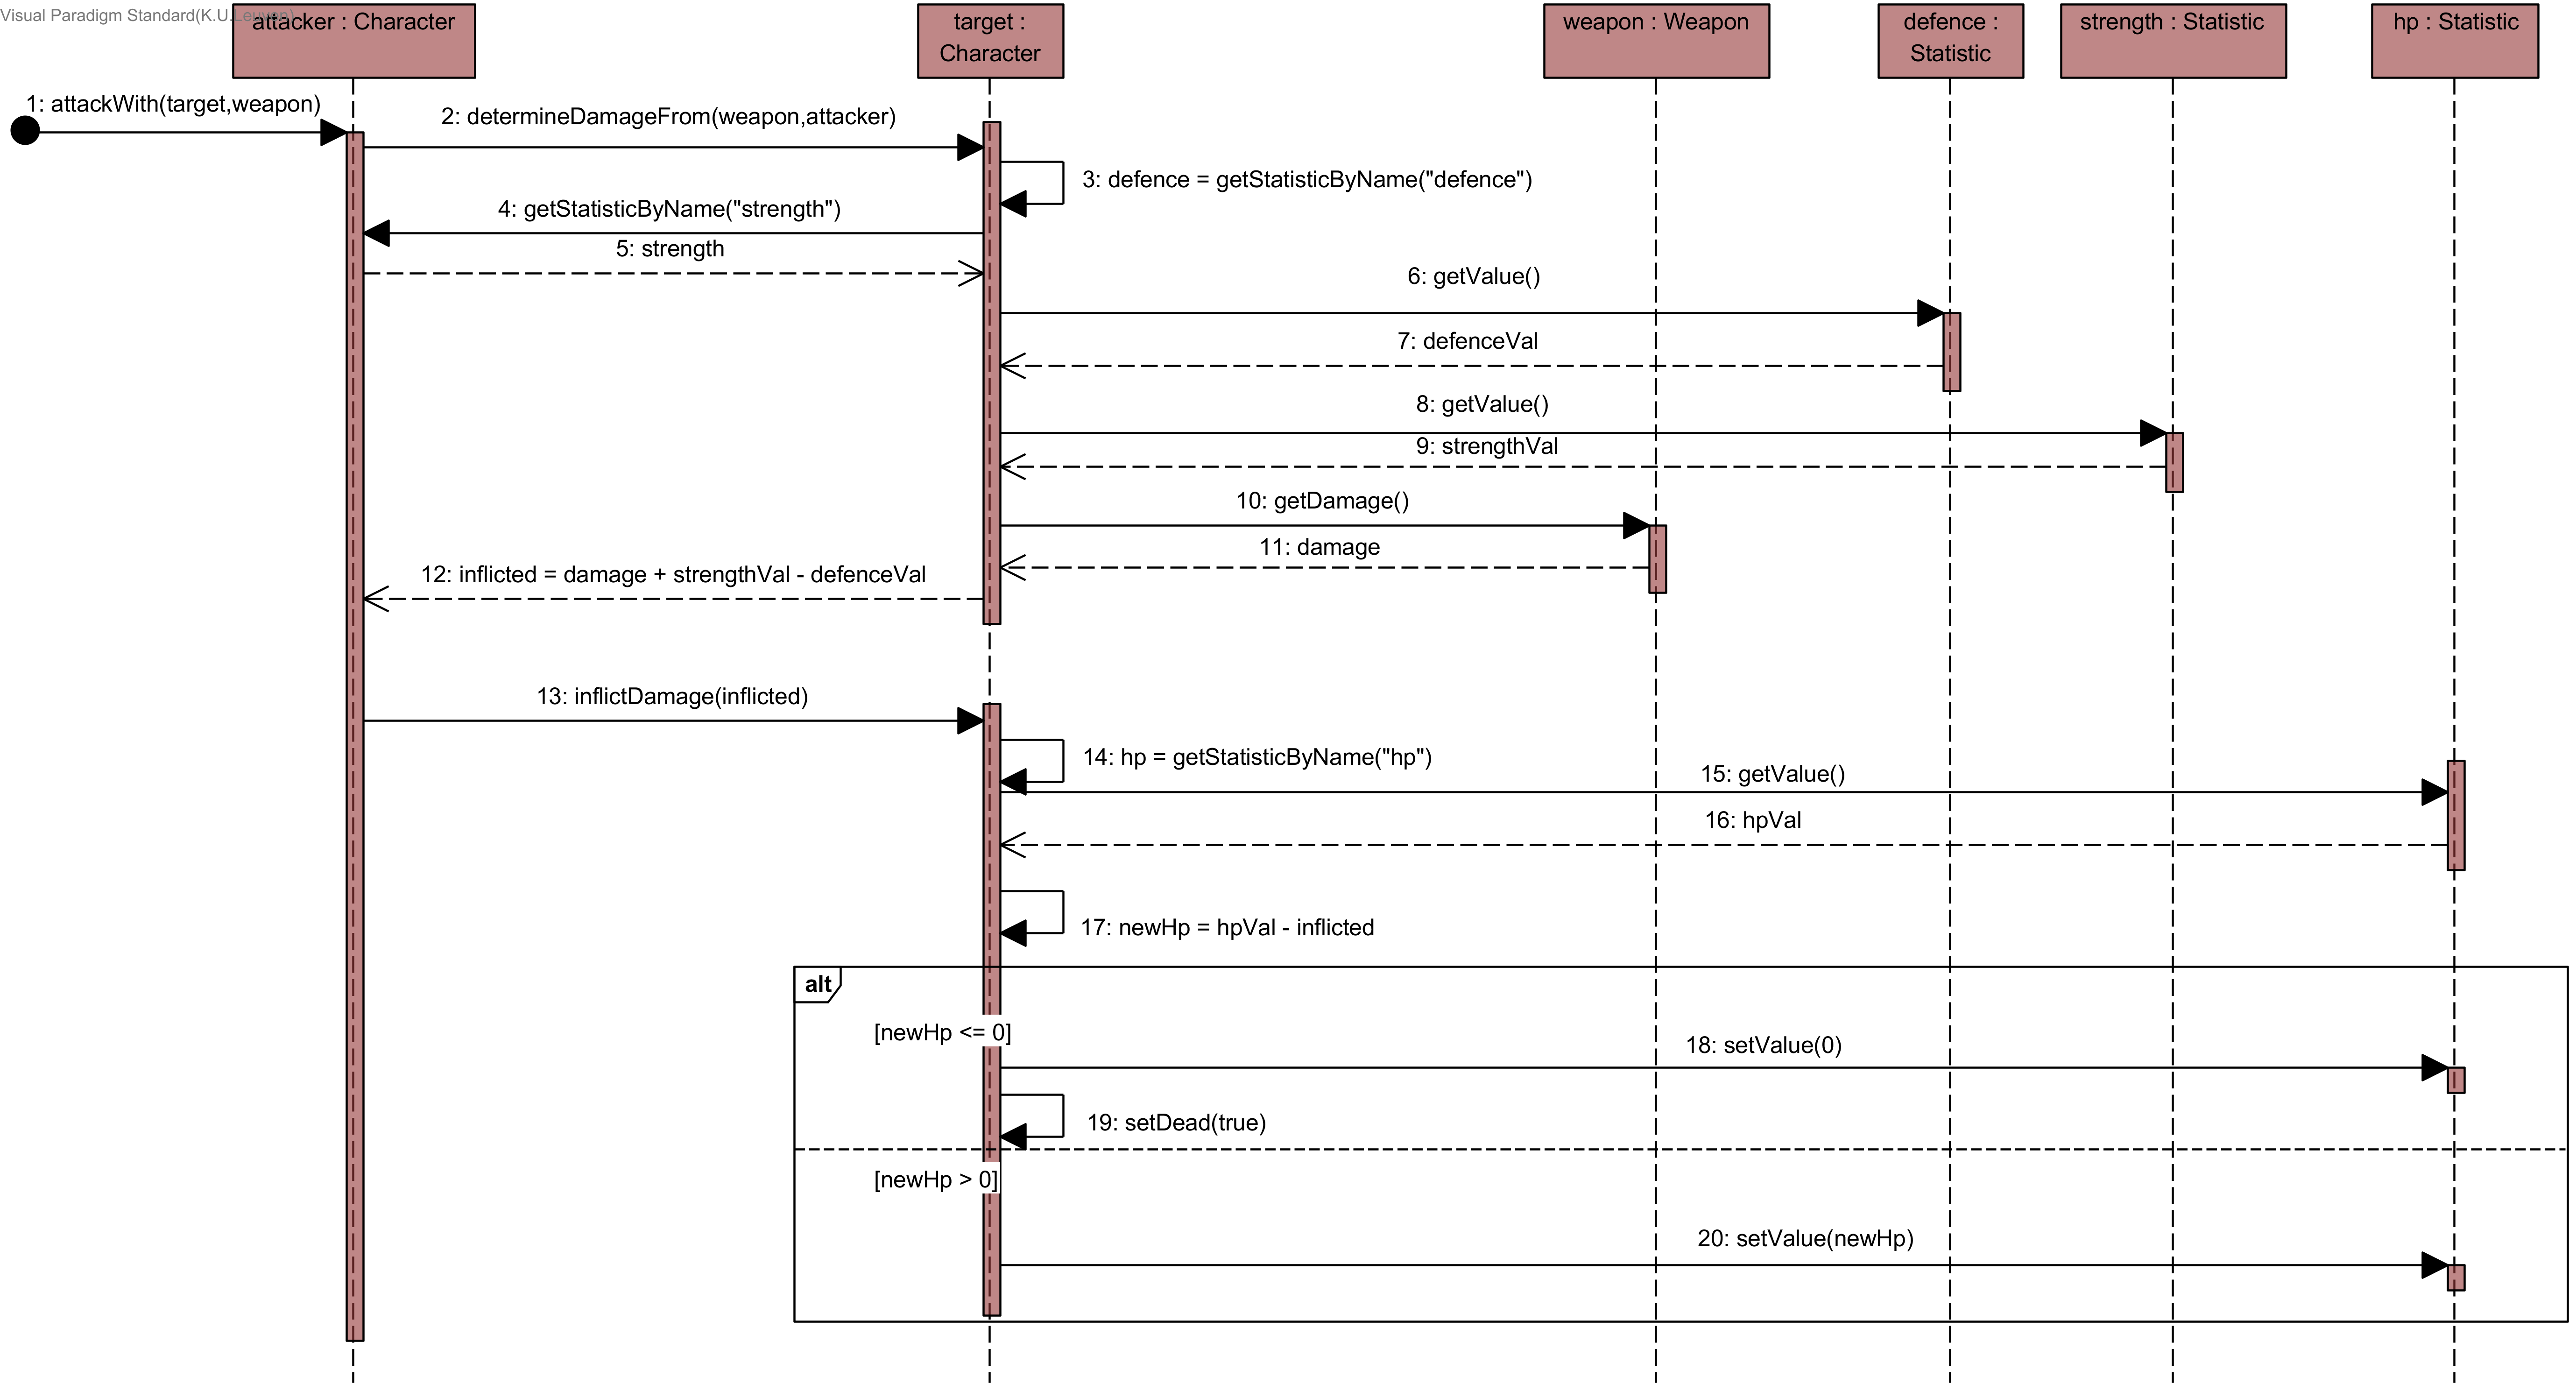
\includegraphics[height=0.55\textwidth]{chap-gedrag/seq-diagram-game.png}
	\caption{Sequentiediagram gebaseerd op het klassediagram van figuur \ref{fig:diagram-voorbeeld}}
	\label{fig:seq-diagram-game}
\end{sidewaysfigure}
%}
%\end{landscape}

\section{De keuze voor lineaire tijdscalculus}\label{sec:sd-ltc}
UML-diagrammen schrijven mogelijke toestanden van softwaresystemen en acties op deze voor. Die systemen kunnen van toestand veranderen tussen tijdstappen. Sequentiediagrammen zijn een manier om te beschrijven hoe zulke veranderingen teweeggebracht kunnen worden. Tijdens de uitvoering van een sequentiediagram mag het systeem enkel veranderen zoals beschreven door de huidige actie. Daarom hebben we een mechanisme nodig binnen FO($\cdot$) dat dynamische systemen en bewerkingen erop kan beschrijven. Tegelijk moet dat mechanisme garanderen dat eigenschappen van het systeem die niet worden be\"invloed door de huidige beschouwde actie van het sequentiediagram niet veranderen. Lineaire tijdscalculus\cite{BogaertsBart2014Sdsu}, oftewel LTC, voldoet aan deze voorwaarden. Daarom zullen we om sequentiediagrammen uitvoerbaar te maken binnen FO($\cdot$) het generatieproces voor het vocabularium en de theorie die we bekomen hebben in hoofdstuk \ref{sec:consistentie} uitbreiden volgens de principes van LTC. Dit betekent dat we de predicaten voor operaties die voorheen gegenereerd werden in hoofdstuk \ref{sec:consistentie} achterwege laten.

In de volgende secties werken we deze uitbreiding uit voor het sequentiediagram in figuur \ref{fig:seq-diagram-game}.

\section{Veranderingen aan het vocabularium}\label{sec:sd-voc}
Allereerst verwijderen we alle predicaten omtrent methodes gegenereerd volgens de regels in sectie \ref{sec:cons-method}. Sequentiediagrammen modelleren immers het gedrag van methodes gedefinieerd in een bijhorend klassediagram, dus zijn deze predicaten nu overbodig.

In LTC is tijd een centraal concept, dus daarom introduceren we een logisch type $Time \subset \mathbb{N}$. Verder defini\"eren we een parti\"ele functie \textit{Next(Time)} dat voor alle tijdpunten het volgende tijdpunt geeft behalve voor het laatst mogelijke tijdpunt. We defini\"eren ook een constante \textit{Start}, wat het eerst mogelijke tijdpunt aanduidt.

Voor elk tijdpunt is het mogelijk dat er een bepaalde instructie van het sequentiediagram wordt uitgevoerd. We duiden deze instructie aan met zijn volgnummer.
Deze volgnummers gebruiken we als instructieteller, en daarvoor defini\"eren we een logisch type $SDPoint \subset \mathbb{N}$.

Om te garanderen dat de instructievolgorde opgelegd door het sequentiediagram gevolgd wordt, maken we deze instructieteller inertieel en introduceren we deze symbolen:

\begin{itemize}
	\item Het toestandspredicaat: \textit{SDPointAt(Time, SDPoint)}
	\item Het begintoestandspredicaat: \textit{I\_SDPointAt(SDPoint)}
	\item Het causatiepredicaat: \textit{C\_SDPointAt(Time, SDPoint)}
\end{itemize}

We moeten ook de instanties waarop gehandeld wordt in het sequentiediagram kunnen benoemen. Om te garanderen dat de instanties die vernoemd worden altijd verwijzen naar hetzelfde object tenzij een instructie een toekenning doet aan de overeenkomstige variabele, maken we ook de instanties inertieel. Voor \textit{attacker} verkrijgen we dan bijvoorbeeld:

\begin{itemize}
	\item \textit{AttackerT(Time, Character)}
	\item \textit{I\_AttackerT(Character)}
	\item \textit{C\_AttackerT(Time, Character)}
\end{itemize}

Het is ook mogelijk dat in een instructie een variabele intern aan het sequentiediagram wordt gedefinieerd. Zo is er instructie 7 waar een \textit{return}-instructie \textit{defenceVal} definieert en ook instructie 12 die de waarde van \textit{inflicted} definieert als een som van andere variabelen. Deze variabelen willen we ook kunnen benoemen en maken we inertieel. Voor alle zulke variabelen defini\"eren we ook predicaten zoals hierboven voor \textit{attacker}.

We passen ook de predicaten die overeenkomen met klasseattributen aan. Het kan immers zijn dat de waarde van een attribuut wordt aangepast, zoals in instructie 18 die de waarde van \textit{value} van object \textit{hp} van klasse \textit{Statistic} verandert naar 0. Klasseattributen maken we ook inertieel. Voor \textit{value} in \textit{Statistic} krijgen we dan:

\begin{itemize}
	\item \textit{Statisticvalue(Time, Statistic, LimitedInt)}
	\item \textit{I\_Statisticvalue(Statistic, LimitedInt)}
	\item \textit{C\_Statisticvalue(Time, Statistic, LimitedInt)}
	\item En het oncausatiepredicaat: \textit{Cn\_Statisticvalue(Time, Statistic, LimitedInt)}
\end{itemize}

Hier voegen we een oncausatiepredicaat toe omdat het mogelijk is dat een attribuut meer dan \'e\'en waarde heeft op een bepaald tijdstip als de bovengrens voor de multipliciteit groter is dan \'e\'en. Met dit predicaat geven we aan dat bepaalde waardes die voor een bepaalde tijdstap gelden ongedaan moeten worden gemaakt in de volgende tijdstap.

\section{Uitbreiden van de theorie}
Voor elke inerti\"ele eigenschap van het systeem moeten er twee dingen gebeuren: Toestandszinnen opstellen en voorwaardes voor causatiezinnen en oncausatiezinnen specificeren. Het resultaat is een inductieve definitie die de inerti\"ele predicaten definieert en een inductieve definitie die de causatiepredicaten en oncausatiepredicaten definieert.

\subsection{Toestandszinnen opstellen}
Toestandszinnen worden geschreven in termen van begintoestandspredicaten, causatiepredicaten en oncausatiepredicaten. Ze garanderen dat inerti\"ele eigenschappen enkel veranderen wanneer het ook echt de bedoeling is dat ze veranderen.

Als eerste kijken we naar toestandszinnen voor \textit{SDPointAt/2}. \textit{I\_SDPointAt/1} geeft aan welke de eerste instructie is die we willen uitvoeren, en daarom schrijven we een definitie die deze overeenkomst uitdrukt:

\begin{align}
	\forall{s}[SDPoint](SDPointAt(Start, s) \leftarrow I\_SDPointAt(s)).
\end{align}


De volgende definities gebruiken het causatiepredicaat:

\begin{align}
	\forall{t}[Time]\forall{s}[SDPoint](SDPointAt(Next(t), s) \leftarrow C\_SDPointAt(Next(t), s)). \label{eq:sdcauses}
\end{align}
\begin{align}
	\forall{t}[Time]\forall{s}[SDPoint](SDPointAt(Next(t), s) \leftarrow SDPointAt(t, s) \nonumber \\ \land{} \space \lnot{}(\exists{s1}[SDPoint](C\_SDPointAt(Next(t), s1)))). \label{eq:sduncauses}
\end{align}

Zin \ref{eq:sduncauses} zorgt ervoor dat de huidige waarde van \textit{SDPointAt} wordt behouden tenzij er een oorzaak is voor verandering.

We schrijven gelijkaardige definities voor de predicaten die overeenkomen met instanties die vernoemd worden in het sequentiediagram (zoals \textit{attacker}).

\parbreak

Voor klasseattributen verloopt dit ook gelijkaardig, maar we wijken af van het formaat van zin \ref{eq:sduncauses} door als volgt het oncausatiepredicaat te gebruiken:

\begin{align*}
	\forall{t}[Time]\forall{s}[Statistic]\forall{i}[LimitedInt](Statisticvalue(Next(t), s, i) \\ \leftarrow Statisticvalue(t, s, i) \land \lnot Cn\_Statisticvalue(Next(t), s, i)).
\end{align*}

\subsubsection{Voorwaardes voor causatie en oncausatie}
We kijken eerst naar klasseattributen. Een aantal ervan worden niet aangepast, wat we bijvoorbeeld neerschrijven voor \textit{range} in \textit{Weapon} als volgt:

\begin{align*}
	\forall{t}[Time]\forall{w}[Weapon]\forall{i}[LimitedInt](C\_Weaponrange(t, w, i) \leftarrow false).
\end{align*}
\begin{align*}
	\forall{t}[Time]\forall{w}[Weapon]\forall{i}[LimitedInt](Cn\_Weaponrange(t, w, i) \leftarrow false).
\end{align*}

Voor de klasseattributen die wel worden aangepast, kijken we naar de instructies die zulke aanpassingen doorvoeren. Voor \textit{value} in \textit{Statistic} zijn dit instructie 18 en 20. We kijken eerst naar de causatiezin en oncausatiezin die volgen uit instructie 18:

\begin{align*}
	\forall{t}[Time]\forall{s}[Statistic](C\_Statisticvalue(t, s, 0) \leftarrow SDPointAt(t, 18) \land HpT(t, s).
\end{align*}
\begin{align*}
	\forall{t}[Time]\forall{s}[Statistic]\forall{i}[LimitedInt](Cn\_Statisticvalue(Next(t), s, i) \\ \leftarrow SDPointAt(Next(t), 18) \land HpT(t, s) \land Statisticvalue(t, s, i) \land \lnot{}(i = 0).
\end{align*}

Aangezien in instructie 18 de instantie \textit{hp} wordt aangesproken, gebruiken we \textit{HpT/2} om te verzekeren dat de waarde van het juiste logisch object wordt veranderd. \textit{value} kan ook maar \'e\'en waarde tegelijk hebben, en daarom schrijven we een oncausatiezin om te verzekeren dat de vorige waarde wordt gewist.

Kijken we nu naar de definities die voortvloeien uit instructie 20:

\begin{align*}
	&\forall{t}[Time]\forall{s}[Statistic]\forall{i}[LimitedInt](C\_Statisticvalue(t, s, i) \\ &\leftarrow SDPointAt(t, 20) \land HpT(t, s) \land NewHpT(t, i)).
\end{align*}
\begin{align*}
&\forall{t}[Time]\forall{s}[Statistic]\forall{i}[LimitedInt](Cn\_Statisticvalue(Next(t), s, i) \\ &\leftarrow SDPointAt(Next(t), 20) \land HpT(t, s) \land Statisticvalue(t, s, i) \land \\ &\lnot{}NewHpT(Next(t), i)).
\end{align*}

Het verschil hier is dat we \textit{NewHpT} erbij betrekken omdat we de waarde van \textit{hp} veranderen naar de waarde van \textit{newHp} in plaats van het te veranderen naar 0.

\parbreak

Het volgende waar we naar kijken zijn de causatiezinnen voor \textit{SDPointAt/2}. Wat we hier willen uitdrukken is dat normaal gezien tussen instructies de instructieteller telkens met \'e\'en wordt verhoogd, tenzij een grens van een \textit{if-else}-constructie of een lus is bereikt. In dat geval kan het zijn dat de instructieteller verspringt afhankelijk van de voorwaarde die vernoemd wordt voor zulke constructies.

Voor deze sequentiediagram krijgen we:

\begin{align}
	&\forall{t}[Time]\forall{s}[SDPoint](C\_SDPointAt(Next(t), (s+1) \leftarrow SDPointAt(t, s) \nonumber \\ &\land \lnot{}((s = 17) \lor (s = 19))). \label{eq:sdprog} \\
	&\forall{t}[Time](C\_SDPointAt(Next(t), 18) \leftarrow SDPointAt(t, 17) \land \nonumber \\ &(\exists{i}[LimitedInt](NewHpT(t, i) \land i <= 0))). \label{eq:sdif} \\
	&\forall{t}[Time](C\_SDPointAt(Next(t), 20) \leftarrow SDPointAt(t, 17 ) \land \nonumber \\ &(\exists{i}[LimitedInt](NewHpT(t, i) \land i > 0))). \label{eq:sdthen} \\
	&\forall{t}[Time](C\_SDPointAt(Next(t), 21) \leftarrow SDPointAt(t, 19) \lor SDPointAt(t, 20)). \label{eq:sdexit}
\end{align}

Zin \ref{eq:sdprog} verzekert het juiste gedrag van de instructieteller, namelijk dat hij doorgaans met \'e\'en wordt verhoogd tussen tijdstappen. De uitzonderingen worden hier ook opgelijst; in dit geval verspringt de teller wanneer men het begin van de \textit{if-else}-constructie tegenkomt en wanneer het einde van het \textit{if}-deel is bereikt. Zinnen \ref{eq:sdif} en \ref{eq:sdthen} controleren de voorwaarde voor de uitvoering van het \textit{if}- en \textit{else}-deel en selecteren wat correct is. Zin \ref{eq:sdexit} zegt dat zowel het \textit{if}-deel als het \textit{else}-deel uitkomen op de instructie die direct volgt op de \textit{if-else}-constructie.

Voor dit diagram is het eenvoudig om deze zinnen op te stellen aangezien er geen geneste gecombineerde fragmenten aanwezig zijn. We beschrijven de algemene methode om het uitvoeringspad doorheen gecombineerde fragmenten te bepalen in sectie \ref{sec:combined-fragment}.

\parbreak

Als laatste zijn er de causatiezinnen voor de verscheidene variabelen die worden aangemaakt en aangesproken in het sequentiediagram. Een aantal van deze variabelen veranderen niet doorheen de uitvoering van het sequentiediagram en er wordt verondersteld dat deze al bekend zijn v\'o\'or de uitvoering begint. Deze variabelen zijn diegenen die betrokken zijn bij de eerste instructie: \textit{attacker}, de instantie die de eerste oproep ontvangt, en \textit{target} en \textit{weapon}, die als parameter worden opgegeven.

Voor de andere variabelen wordt er een causatiezin toegevoegd voor elke instructie die een waarde toekent aan die variabele. Als voorbeeld bekijken we instructie 3:

\begin{align*}
	&\forall{t}[Time]\forall{d}[Statistic](C\_DefenceT(t, d) \leftarrow SDPointAt(t, 3) \land \\ &\exists{c}[Character](TargetT(t, c) \land CharacterandStatistic(c, d) \\ &\land Statisticname(t, d, "defence"))).
\end{align*}


De zin drukt uit dat de getter wordt opgeroepen op \textit{target} en dat er wordt gevraagd naar een instantie van \textit{Statistic} dat in verband staat met \textit{target} en als naam ``defence'' heeft. Die instantie wordt dan als waarde toegekend aan de variabele \textit{defence}.

De volledige uitvoertheorie voor diagram \ref{fig:seq-diagram-game} is beschikbaar op de volgende online locatie: \url{https://pastebin.com/WGQjr2bv}.

\section{Het uitvoeren van gecombineerde fragmenten}\label{sec:combined-fragment}
Het opstellen van causatiezinnen voor \textit{SDPointAt/2} ten gevolge van gecombineerde fragmenten is niet vanzelfsprekend. Deze sectie beschrijft onze methode om dit te bewerkstelligen.
Bij de vertaling van sequentiediagrammen houden we in de interne voorstelling binnen onze vertaler van een gecombineerd fragment volgende zaken bij:

\begin{itemize}
	\item Alle gecombineerde fragmenten die kinderen zijn van het fragment.
	\item Het fragment dat de ouder is van het fragment in kwestie, als die bestaat.
	\item Alle berichten die rechtstreeks deel zijn van het fragment. Een bericht is rechtstreeks deel van een fragment als het bericht een deel is van het fragment, maar geen rechtstreeks deel is van een kind of afstammeling van het fragment.
	\item De voorwaarde waaraan voldaan moet zijn om het fragment uit te voeren. 
\end{itemize}

Voor alt-fragmenten maken we het onderscheid tussen kinderen en berichten van het \textit{if}-gedeelte enerzijds en tussen kinderen en berichten van het \textit{else}-gedeelte anderzijds. Ook geldt dat er een voorwaarde is voor de uitvoering van het \textit{if}-gedeelte en voor de uitvoering van het \textit{else}-gedeelte.

In de methode om in de uitvoertheorie het uitvoeringspad doorheen gecombineerde fragmenten correct te vertalen gebruiken we drie procedures: E\'en die bepaalt naar welke berichten wordt gesprongen onder welke voorwaarde bij het binnengaan van een fragment, \'e\'en die bepaalt naar welke berichten wordt gesprongen onder welke voorwaarde bij het buitengaan van een fragment en \'e\'en die de heruitvoering van een lus verzorgt indien de voorwaarde voor de lus nog geldt. We bespreken deze procedures afzonderlijk.

\subsection{Transitie naar een fragment}\label{sec:transition-to}

Het resultaat van deze procedure is een mapping van berichten waarnaar gesprongen kan worden bij het binnengaan van een fragment naar onder welke voorwaarde deze sprong gebeurt. We willen dat deze procedure dit niet enkel doet voor het gegeven fragment, maar ook voor alle kinderen van het fragment. Op die manier worden alle fragmenten verwerkt wanneer de procedure wordt opgeroepen voor alle fragmenten zonder ouders.
We geven een overzicht van de procedure in algoritme \ref{alg:transition-to-frag}.

\parbreak

\begin{algorithm}
	\KwIn{\textit{fragment : gecombineerd fragment}; \textit{aggregateVoorwaarde : string}}
	\KwOut{Een mapping van bericht naar string. De string stelt de voorwaarde voor waaronder naar een bericht wordt gesprongen bij de transitie naar een fragment.}
	$uitvoer \leftarrow \emptyset$; \\
	\textit{gezien $\leftarrow \emptyset$}; \\
	\eIf{eerste bericht is rechtstreeks deel van fragment}{
	$uitvoer \leftarrow uitvoer $\textit{ + \{eerste bericht $\rightarrow$ aggregateVoorwaarde + voorwaarde voor fragment\}}; \\
	\textit{kinderen $\leftarrow$ kinderen van fragment}; \\
	\textit{uitvoer $\leftarrow$ uitvoer $\cup$ vouwLussen(gezien, kinderen, $\epsilon$, \textbf{false}, \textbf{true})}; zie algoritme \ref{alg:wrap-loops} \\
	\ForEach{kind $\in$ kinderen}{
		\If{kind $\notin$ gezien}{
		\textit{uitvoer $\leftarrow$ uitvoer $\cup$ bepaalTransitieIn(kind, ``'')};}}
	 }{
	 \textit{eersteFragment $\leftarrow$ eerste kind van fragment}; \\
	 \eIf{eersteFragment is lusfragment}{
	 	\textit{voorwaarde $\leftarrow$ aggregateVoorwaarde + ``$\land$'' + voorwaarde voor fragment}; \\
	 	\textit{uitvoer $\leftarrow$ uitvoer $\cup$ bepaalTransitieIn(eersteFragment, voorwaarde)}; \\
	 	\textit{voorwaarde $\leftarrow$ voorwaarde + ``$\land \lnot$('' + voorwaarde voor eersteFragment + ``)''}; \\
	 	\textit{kinderen $\leftarrow$ kinderen van fragment}; \\
	 	\textit{uitvoer $\leftarrow$ uitvoer $\cup$ vouwLussen(gezien, kinderen, voorwaarde, \textbf{true}, \textbf{true})};
	 }{
	 \textit{voorwaarde $\leftarrow$ aggregateVoorwaarde + ``$\land$'' + voorwaarde voor fragment}; \\
	 \textit{uitvoer $\leftarrow$ uitvoer $\cup$ bepaalTransitieIn(eersteFragment, voorwaarde)};
 	}
 	\ForEach{kind $\in$ kinderen}{
 		\If{kind $\notin$ gezien}{
 		\textit{uitvoer $\leftarrow$ uitvoer $\cup$ bepaalTransitieIn(kind, ``'')};}
 	}
	}
	\textbf{return} \textit{uitvoer};
	\caption{bepaalTransitieIn}
	\label{alg:transition-to-frag}
\end{algorithm}

\begin{algorithm}
	\KwIn{\textit{gezien : verzameling van gecombineerde fragmenten}; \textit{kinderen : lijst van gecombineerde fragmenten}; \textit{aggregateVoorwaarde : string}; \textit{slaEersteOver : boolean}; \textit{allemaal : boolean}}
	\KwOut{Een mapping van bericht naar string, zoals in algoritme \ref{alg:transition-to-frag}}
	\textit{uitvoer $\leftarrow \emptyset$}; \\
	\ForEach{\textit{kind} $\in$ \textit{kinderen}}{
	\eIf{kind is lusfragment}{
	\eIf{allemaal}{
	\textit{uitvoer $\leftarrow$ uitvoer $\cup$ bepaalTransitieIn(kind, aggregateVoorwaarde)};
	}{
	\textit{uitvoer $\leftarrow$ uitvoer $\cup$ bepaalTransitieInOnvolledig(kind, aggregateVoorwaarde)};
	}
	\textit{aggregateVoorwaarde} $\leftarrow$ \textit{aggregateVoorwaarde + ``$\land{} \lnot$('' + voorwaarde voor kind + ``)''}; \\
	\textit{gezien $\leftarrow$ gezien + kind};
	}{
	\eIf{$\lnot$ allemaal}{
	\textbf{break};}{
	\textit{aggregateVoorwaarde} $\leftarrow \epsilon$;}
	}}
	\textbf{return} \textit{uitvoer};
	\caption{vouwLussen}
	\label{alg:wrap-loops}
\end{algorithm}

In algoritme \ref{alg:wrap-loops} is \textit{bepaalTransitieInOnvolledig} een variant van \textit{bepaalTransitieIn} waar er geen recursieve oproep is voor die kinderen die niet betrokken zijn in het vouwproces voor lusfragmenten.

Merk op dat voor alt-fragmenten algoritme \ref{alg:transition-to-frag} wordt uitgevoerd voor het \textit{if}-gedeelte en het \textit{else}-gedeelte afzonderlijk.

De kern van algoritme \ref{alg:transition-to-frag} is dat in de uitvoertheorie in \'e\'en stap bepaald moet worden welk bericht eerst zal worden uitgevoerd wanneer het uitvoerpad een gecombineerd fragment binnengaat. Daarom bouwen we doorheen de recursie een aggregate voorwaarde op die bestaat uit een conjunctie van voorwaarden voor fragmenten. Enkel wanneer een fragment bereikt wordt waarvoor geldt dat het eerste bericht rechtstreeks deel is van dat fragment wordt er een mapping van dat bericht naar die aggregate voorwaarde toegevoegd. Hierna maken we de aggregate voorwaarde terug leeg om dan het proces voort te zetten voor de kinderen.

Algoritme \ref{alg:wrap-loops} is nodig omdat lusfragmenten die elkaar opvolgen een speciaal geval vormen. Voor een lusfragment geldt immers dat het wordt uitgevoerd indien de voorwaarde voor dat lusfragment vervuld is en de voorwaarden voor alle voorgaande lusfragmenten niet vervuld zijn. Figuur \ref{fig:seq-diagram-frag-ex} stelt bijvoorbeeld dat de uitvoering springt naar de lus aangeduid met \fragname{loop4} als aan de voorwaarde voor de lus aangeduid met \fragname{loop3} niet voldaan is. Algoritme \ref{alg:wrap-loops} markeert alle fragmenten die het voor zijn rekening neemt zodat ze niet opnieuw worden behandeld in algoritme \ref{alg:transition-to-frag}.

\subsection{Transitie uit een fragment}\label{sec:transitions-out}

Het doel is om te bepalen welke berichten dienen als punten waar het uitvoerpad een gecombineerd fragment verlaat (verder een `verlaatpunt'), en naar welke berichten de uitvoer springt onder welke voorwaarden. Daarom is het resultaat van deze procedure een mapping van verlaatpunt naar een verzameling van paren van bericht en voorwaarde die moet gelden om naar dat bericht te springen. We geven een overzicht van de procedure in algoritme \ref{alg:calcExitForMessages}.

\begin{algorithm}
	\thispagestyle{empty}
	\KwIn{\textit{fragment : gecombineerd fragment; uitvoer : lege verzameling van bericht $\rightarrow$ verzameling van \{bericht $\rightarrow$ string\}}}
	\KwOut{\textit{Verzameling van bericht $\rightarrow$ \{bericht $\rightarrow$ string\}}}
	\textit{\{laatsteBericht, aggregateVoorwaarde\} $\leftarrow$ bepaalLaatsteBericht(fragment)}; zie algoritme \ref{alg:determineFinalMessage} \\
	\If{laatsteBericht is niet leeg}{
	\textit{mapPaar $\leftarrow \emptyset$}; \\
	\eIf{fragment heeft geen ouder}{
	\textit{transitieNaarBuiten(fragment, mapPaar, (negatie van lusvoorwaarde als fragment een lusfragment is, anders $\epsilon$))}; zie algoritme \ref{alg:exitToOutside} \\
	\textit{uitvoer $\leftarrow$ uitvoer + (laatsteBericht $\rightarrow$ mapPaar)};}{
	\textit{concateneer aggregateVoorwaarde met negatie van lusvoorwaarde voor fragment als fragment een lus is} \\
	\textit{fragment $\leftarrow$ ouder van fragment}; \\
	\If{bericht na laatsteBericht is deel van fragment}{
	\textit{berichtNa $\leftarrow$ bericht na laatsteBericht}; \\
	\textit{kind $\leftarrow$ voorouder van fragment waar berichtNa rechtstreeks deel van is dat fragment als ouder heeft}; \\
	\textit{kinderenNa $\leftarrow$ \{kind\} $\cup$ alle kinderen van fragment die na kind komen}; \\
	\textit{als het eerste lid van kinderenNa geen lusfragment is, hou enkel dat eerste lid over; anders, hou eerste lid, alle lusfragmenten die meteen volgen op het eerste lid, en het meteen daaropvolgende fragment, als er \'e\'en is, over} \\
	\textit{transitiesIn $\leftarrow \emptyset$}; \\
	\ForEach{kindFragment $\in$ kinderenNa}{
	\textit{negaties $\leftarrow$ conjunctie van negaties van lusvoorwaarden van voorgaande lussen als die er zijn, anders ``''}; \\
	\textit{transitiesIn $\leftarrow$ transitiesIn $\cup$ bepaalTransitiesIn(kindFragment, negaties)}; \\}
	\textit{concateneer alle sprongvoorwaarden in transitiesIn met aggregateVoorwaarde} \\
	\textit{voeg alle elementen van transitiesIn toe aan mapPaar} \\
	\textit{uitvoer $\leftarrow$ uitvoer + (laatsteBericht $\rightarrow$ mapPaar);} \\
	\textit{ga naar stap 31 als het laatste lid van kinderenNa geen lus is, anders naar stap 23}}
	\eIf{fragment heeft een ouder}{
	\textit{concateneer aggregateVoorwaarde met negatie van lusvoorwaarde voor fragment als fragment een lus is} \\
	\textit{fragment $\leftarrow$ ouder van fragment;} \\
	\textit{ga naar stap 10}}{
	\textit{transitieNaarBuiten(fragment, mapPaar, aggregateVoorwaarde)}; \\
	\textit{uitvoer $\leftarrow$ uitvoer + (laatsteBericht $\rightarrow$ mapPaar)}; \\
	\textit{ga naar stap 31}}
	}
	}
	\ForEach{kind $\in$ kinderen van fragment dat initieel als argument werd gegeven}{
	\textit{bepaalTransitieUit(kind, uitvoer)}}
	\textbf{return};
	\caption{bepaalTransitieUit}
	\label{alg:calcExitForMessages}
\end{algorithm}

\begin{algorithm}
	\KwIn{fragment : gecombineerd fragment}
	\KwOut{Paar van bericht en string}
	\textit{aggregateVoorwaarde $\leftarrow \epsilon$}; \\
	\textit{containers $\leftarrow$ gesorteerde lijst van berichtcontainers van fragment}; \tcc{een berichtcontainer is ofwel \'e\'en enkel bericht of een gecombineerd fragment---op deze manier kunnen we een gecombineerd fragment beschouwen als een verzameling van berichtcontainers die bestaat uit de berichten die rechtstreeks deel zijn van het fragment en de kinderen van het fragment}
	\ForEach{container $\in$ containers, beginnend vanaf de laatste}{
	\If{container is een bericht}{
	\textbf{return} \textit{\{container, aggregateVoorwaarde\}};
	}
	\eIf{container is geen lus}{
	\textbf{return} \textit{\{$\emptyset$, aggregateVoorwaarde\}};}
	{
	\textit{aggregateVoorwaarde $\leftarrow$ aggregateVoorwaarde + ``$\land \lnot$('' + lusvoorwaarde van container + ``)''};
	}}
	\textbf{return} \textit{\{$\emptyset$, $\epsilon$\}};
	\caption{bepaalLaatsteBericht}
	\label{alg:determineFinalMessage}
\end{algorithm}

\begin{algorithm}
	\KwIn{\textit{fragment : gecombineerd fragment; mapPaar : verzameling van \{bericht $\rightarrow$ string\}; transitieVoorwaarde : string}}
	\If{bericht meteen na dit fragment is deel van een lusfragment zonder ouder}{
	\textit{volgenden $\leftarrow$ alle lussen die meteen volgen op fragment en het meteen daaropvolgende fragment, als er \'e\'en is}; \\
	\textit{aggregateVoorwaarde $\leftarrow \epsilon$}; \\
	\ForEach{volgendFragment $\in$ volgenden}{
	\textit{transitiesIn $\leftarrow$ bepaalTransitieIn(volgendFragment, aggregateVoorwaarde)}; \\
	\textit{concateneer alle sprongvoorwaarden in transitiesIn met transitieVoorwaarde}; \\
	\textit{mapPaar $\leftarrow$ mapPaar $\cup$ transitiesIn}; \\
	\If{volgendFragment is een lusfragment}{\textit{aggregateVoorwaarde $\leftarrow$ aggregateVoorwaarde + ``$\land \lnot$('' + voorwaarde voor lus + ``)''};}}
	\If{laatste lid van volgenden is geen lus}{
	\textbf{return};}
	}
	\textit{volgend $\leftarrow$ bericht dat meteen volgt op fragment}; \\
	\If{volgend is deel van gecombineerd fragment}{
	\textit{topFragment $\leftarrow$ voorouder van fragment waar volgend deel van is die zelf geen ouder heeft}; \\
	\textit{transitiesIn $\leftarrow$ bepaalTransitieIn(topFragment, ``'')}; \\
	\textit{concateneer alle sprongvoorwaarden in transitiesIn met transitieVoorwaarde}; \\
	\textit{mapPaar $\leftarrow$ mapPaar $\cup$ transitiesIn}; \\
	\textbf{return};}
	\textit{mapPaar $\leftarrow$ mapPaar + \{volgend $\rightarrow$ transitieVoorwaarde\}}; \\
	\textbf{return};
	\caption{transitieNaarBuiten}
	\label{alg:exitToOutside}
\end{algorithm}

Merk op in stap 3 dat \textit{laatsteBericht} later wordt gemapt naar een mapping van berichten naar de voorwaarde waaronder naar die berichten wordt gesprongen vanaf \textit{laatsteBericht}.
Algoritme \ref{alg:calcExitForMessages} gebruikt eerst algoritme \ref{alg:determineFinalMessage} om te bepalen of het laatste bericht van het fragment rechtstreeks deel is ervan. Zoniet, gaat het algoritme voort met de kinderen van het fragment. Zoja, controleren we of het fragment een ouder heeft. Als dat zo is, dan kan het zijn dat die ouder een bericht heeft dat in het diagram meteen na het laatste bericht van het fragment komt en dat het uitvoerpad dus mogelijk naar dat bericht springt. Als dat bericht rechtstreeks deel is van de ouder, dan wordt genoteerd dat de uitvoering vanaf het laatste bericht springt naar dat bericht en gaat het algoritme verder vanaf stap 31 (door ruimtegebrek is deze mogelijkheid niet neergeschreven in deze weergave van algoritme \ref{alg:calcExitForMessages}). Als het bericht in de plaats deel is van een kind van de ouder, haalt het algoritme het fragment op waarvan dat bericht rechtstreeks deel is, klimt het naar boven in de boom tot het een kind van de ouder tegenkomt, bundelt opeenvolgende lussen als dat kind een lusfragment is (en ook het fragment na die lussen, als er \'e\'en bestaat) en roept dan algoritme \ref{alg:transition-to-frag} op op alle gebundelde fragmenten. In de uitvoer wordt dan genoteerd dat het uitvoerpad kan springen naar de berichten die deel zijn van de uitvoer van algoritme \ref{alg:transition-to-frag}. Als op het laatste lusfragment een bericht volgt in plaats van een ander type fragment, noteren we dat naar dat bericht kan worden gesprongen (deze mogelijkheid staat niet in het algoritme door ruimtegebrek). Het algoritme gaat verder met de kinderen van het oorspronkelijk fragment.

Als het bericht na het laatste bericht geen deel is van de ouder, of als het laatste lid van \textit{kinderenNa} een lus is, of als het laatste lid van \textit{kinderenNa} geen lus is en er volgt geen bericht op, controleren we of de ouder zelf een ouder heeft. Zoja, neemt het algoritme een stap naar boven in de fragmentenboom. Bij deze stap markeren we eerst het huidige fragment zodat deze niet meer beschouwd wordt in verdere oproepen van algoritme \ref{alg:transition-to-frag} en concateneren we \textit{aggregateVoorwaarde} met de negaties van de lusvoorwaardes van de lussen op het einde van het fragment, als die er zijn (niet weergegeven in algoritme door plaatsgebrek). Zonee, betekent dit dat de top van de fragmentenboom is bereikt en dat het uitvoerpad de boom moet verlaten. Algoritme \ref{alg:exitToOutside} zorgt voor deze stap uit de boom. We controleren of de fragmentenboom wordt opgevolgd door een lusfragment en bundelen alle volgende lusfragmenten (en het meteen daaropvolgend fragment, als er \'e\'en bestaat) als dat zo is. We roepen algoritme \ref{alg:transition-to-frag} op met die fragmenten om de beurt als argument en registreren de uitvoer als berichten waarnaar gesprongen kan worden. Als er geen lus volgt op de boom, roepen we algoritme \ref{alg:transition-to-frag} op als er een fragment volgt, en anders noteren we het bericht dat meteen volgt op de boom als een bericht waarnaar gesprongen kan worden.

Merk op dat voor alt-fragmenten algoritme \ref{alg:calcExitForMessages} afzonderlijk wordt uitgevoerd voor het \textit{if}-gedeelte en het \textit{else}-gedeelte afzonderlijk.

\subsection{Het herhaaldelijk uitvoeren van een lus}\label{sec:loop-reentry}
Een laatste aspect is dat we ervoor moeten zorgen dat een lus terug wordt uitgevoerd als de laatste instructie bereikt is en de lusvoorwaarde nog geldt. We gebruiken algoritme \ref{alg:calculateLoopReentry} om te bepalen vanaf welke berichten terug wordt gesprongen naar de mogelijke beginpunten van een lusfragment.

\begin{algorithm}
	\KwIn{fragment : gecombineerd fragment}
	\KwOut{Verzameling van bericht $\rightarrow$ \{bericht $\rightarrow$ string\}}
	\textit{uitvoer $\leftarrow \emptyset$}; \\
	\textit{uitgesloten $\leftarrow \emptyset$}; \\
	\textit{aggregateVoorwaarde $\leftarrow \epsilon$}; \\
	\ForEach{laatsteBericht $\in$ mogelijke laatste berichten van fragment}{
	\Do{fragment heeft een ouder}{
	\If{fragment is een lusfragment en laatsteBericht is een mogelijk laatst bericht van fragment}{
	\textit{containers $\leftarrow$ containers van fragment}; \\
	\eIf{eerste container is lus}{
	\textit{bundelVoorwaarde $\leftarrow$ voorwaarde van lus als de laatste container een fragment is en laatsteBericht is daar een laatste bericht van, anders $\epsilon$}; \\
	\ForEach{container $\in$ containers}{
	\eIf{container is een fragment en container $\notin$ uitgesloten}{
	\textit{transities $\leftarrow$ bepaalTransitieInOnvolledig(fragment, $\epsilon$, uitgesloten)}; \\
	\textit{concateneer alle sprongvoorwaardes in transities met aggregateVoorwaarde en bundelVoorwaarde}; \\
	\ForEach{bericht---voorwaarde-paar $\in$ transities}{
	\textit{uitvoer $\leftarrow$ uitvoer + \{laatsteBericht $\rightarrow$ \{bericht $\rightarrow$ voorwaarde\}\}};
	}
	}{
	\textit{uitvoer $\leftarrow$ uitvoer + \{laatsteBericht $\rightarrow$ \{container $\rightarrow$ aggregateVoorwaarde + bundelVoorwaarde\}\};}
	}
	\eIf{container is een lus}{
	\textit{bundelVoorwaarde $\leftarrow$ bundelVoorwaarde + ''$\land \lnot$(``voorwaarde voor container + ``)''};
	}{
	\textbf{break};}
	}}
	{
	\textit{transities $\leftarrow$ bepaalTransitieInOnvolledig(fragment, $\epsilon$, uitgesloten)}; \\
	\textit{concateneer alle sprongvoorwaardes in transities met aggregateVoorwaarde}; \\
	\ForEach{bericht---voorwaarde-paar $\in$ transities}{
		\textit{uitvoer $\leftarrow$ uitvoer + \{laatsteBericht $\rightarrow$ \{bericht $\rightarrow$ voorwaarde\}\}};
	}
	}
	}
	\If{fragment is een lusfragment}{
	\textit{uitgesloten $\leftarrow$ uitgesloten + fragment};}
	\If{fragment heeft een ouder}{
	\If{fragment is een lusfragment}{\textit{aggregateVoorwaarde $\leftarrow$ aggregateVoorwaarde + ``$\land \lnot$('' + voorwaarde voor lusfragment + ``)''};}
	\textit{fragment $\leftarrow$ ouder van fragment};
	}}}
	\caption{bepaalLusHeruitvoering}
	\label{alg:calculateLoopReentry}
\end{algorithm}

We gebruiken hier een variant van \textit{bepaalTransitieInOnvolledig} waarbij de fragmenten doorgegeven in \textit{uitgesloten} worden overgeslagen.
De mogelijke laatste berichten van een fragment zijn deze waarbij het uitvoerpad het fragment verlaat nadat ze zijn uitgevoerd, bijvoorbeeld de laatste berichten van de \textit{if}- en \textit{else}-gedeeltes van een alt-fragment of een bericht dat voorafgaat aan een lusfragment.

Vanaf zulk een laatste bericht gaan we van onderaf naar boven in de boom, beginnend bij het fragment dat als argument wordt gegeven van de oproep. Telkens we een lusfragment tegenkomen waarvan dat bericht een laatste bericht is, moeten we voor dat fragment alle mogelijke beginpunten vinden. We beschouwen de \textit{containers} voor het fragment. Indien de eerste \textit{container} een lus is, controleren we of de laatste \textit{container} een lus is en of \textit{laatsteBericht} een laatst bericht ervan is. In dat geval moeten we verzekeren dat er rekening wordt gehouden met de lusvoorwaarde van de lus op dit niveau wanneer we \textit{bepaalTransitieInOnvolledig} gebruiken. Verder gaan we de \textit{containers} af: We bundelen de negaties van de voorwaardes van voorafgaande lusfragmenten samen, we bepalen de transitiepunten ervan en we gaan naar boven in de boom nadat we een \textit{container} zijn tegengekomen die geen lus is of als we alle \textit{containers} hebben beschouwd.

Als de eerste \textit{container} geen lus is, bepalen we de transitiepunten van het fragment en gaan dan naar boven in de boom.

\subsection{De vertaling van transities}\label{sec:process-frag}

Nu volgt een beschrijving van hoe we de voorgaande algoritmes gebruiken om een verzameling van mappings van berichten waarnaar gesprongen wordt naar een mapping van berichten waarvan gesprongen wordt en onder welke voorwaarde vanaf die berichten wordt gesprongen bij te houden. We geven een beschrijving op hoog niveau in algoritme \ref{alg:processCombinedFragment}. Bij de uitvoering ervan werken we vanuit de veronderstelling dat alle berichten en fragmenten van een diagram toegankelijk zijn.

\begin{algorithm}
	\KwIn{fragment : gecombineerd fragment; uitvoer : verzameling van bericht $\rightarrow$ verzameling van \{bericht $\rightarrow$ string\}}
	\If{fragment is een lusfragment, heeft geen ouder en wordt voorgegaan door een bericht dat geen deel is van een gecombineerd fragment}{
	\textit{noteer in uitvoer dat dit fragment en de lussen die er direct op volgen worden overgeslagen als de lusvoorwaarde voor geen enkele ervan geldt}
	}
	\eIf{er is een fragment dat vlak v\'o\'or fragment komt}{
	\textit{vorig $\leftarrow$ fragment dat vlak v\'o\'or fragment komt}; \\
	\textit{verwerkFragment(vorig, uitvoer)}; \\
	\textit{bepaalVerlaatpunten(fragment, uitvoer)}; \\
	\textit{verzekerLusHeruitvoering(fragment, uitvoer)};
	}{
	\textit{transitieIn $\leftarrow$ bepaalTransitieIn(fragment, $\epsilon$)}; \\
	\ForEach{\{bericht---voorwaarde\} $\in$ transitieIn}{
	\textit{berichtVoor $\leftarrow$ bericht dat v\'o\'or bericht komt}; \\
	\eIf{berichtVoor is geen deel van een fragment}{
	\textit{uitvoer $\leftarrow$ uitvoer + \{berichtVoor $\rightarrow$ \{bericht $\rightarrow$ voorwaarde\}\}};
	}
	{
	\textit{vorigFragment $\leftarrow$ fragment waar berichtVoor deel van is}; \\
	\textit{transitiesUit $\leftarrow$ bepaalTransitieUit(vorigFragment);} \\
	\textit{voor alle voorkomens van bericht in transitiesUit als bericht waarnaar gesprongen wordt, doe uitvoer $\leftarrow$ uitvoer + \{sprongbericht $\rightarrow$ \{bericht $\rightarrow$ sprongvoorwaarde horend bij bericht\}\}
	}}
	}
	\textit{bepaalVerlaatpunten(fragment, uitvoer);} \\
	\textit{verzekerLusHeruitvoering(fragment, uitvoer)};
	}
	\caption{verwerkFragment}
	\label{alg:processCombinedFragment}
\end{algorithm}

\textit{bepaalVerlaatPunten} gebruikt algoritme \ref{alg:calcExitForMessages} om te bepalen naar welke berichten wordt gesprongen onder welke voorwaarde vanuit het fragment. \textit{verzekerLusHeruitvoering} bouwt een fragmentenboom op met het gegeven fragment als wortel en roept algoritme \ref{alg:calculateLoopReentry} op met elke knoop in de boom om de beurt als argument om te verzekeren dat lussen worden heruitgevoerd wanneer de lusvoorwaarde nog geldt.

Bij het vertalen van sequentiediagrammen roepen we algoritme \ref{alg:processCombinedFragment} op met alle fragmenten in het diagram om de beurt als argument. De resulterende informatie geeft ons:

\begin{enumerate}
	\item De berichten waarnaar gesprongen wordt
	\item De berichten vanwaar gesprongen wordt
	\item Onder welke voorwaarde zulk een sprong gebeurt
\end{enumerate}

We gebruiken dit om de eigenlijke vertaling van gecombineerde fragmenten naar FO($\cdot$) te bepalen.

\subsection{Voorbeeld van gecombineerd fragment vertaling}

We defini\"eren eerst notatie die we verder gebruiken bij het uitwerken van een voorbeeld:

\begin{align*}
	\transitionentry{\fragcond{voorwaarde}}{\fragmessage{$bericht_a$}}
\end{align*}

Dit betekent dat de uitvoering kan springen naar $bericht_a$ onder \textit{\fragcond{voorwaarde}}.

\begin{align*}
	\transitionentry[\fragmessage{$bericht_b$}]{\fragcond{voorwaarde}}{\fragmessage{$bericht_a$}}
\end{align*}

Dit betekent dat de uitvoering vanaf \fragmessage{$bericht_b$} springt naar \fragmessage{$bericht_a$} onder \textit{\fragcond{voorwaarde}}.

\subsubsection{De uitvoering van de voorgestelde algoritmes}

Deze sectie gebruikt figuur \ref{fig:seq-diagram-frag-ex} om een voorbeeld te geven van de vertaling van gecombineerde fragmenten volgens de algoritmes beschreven in secties \ref{sec:transition-to}, \ref{sec:transitions-out}, \ref{sec:loop-reentry} en \ref{sec:process-frag}.

\begin{figure}
	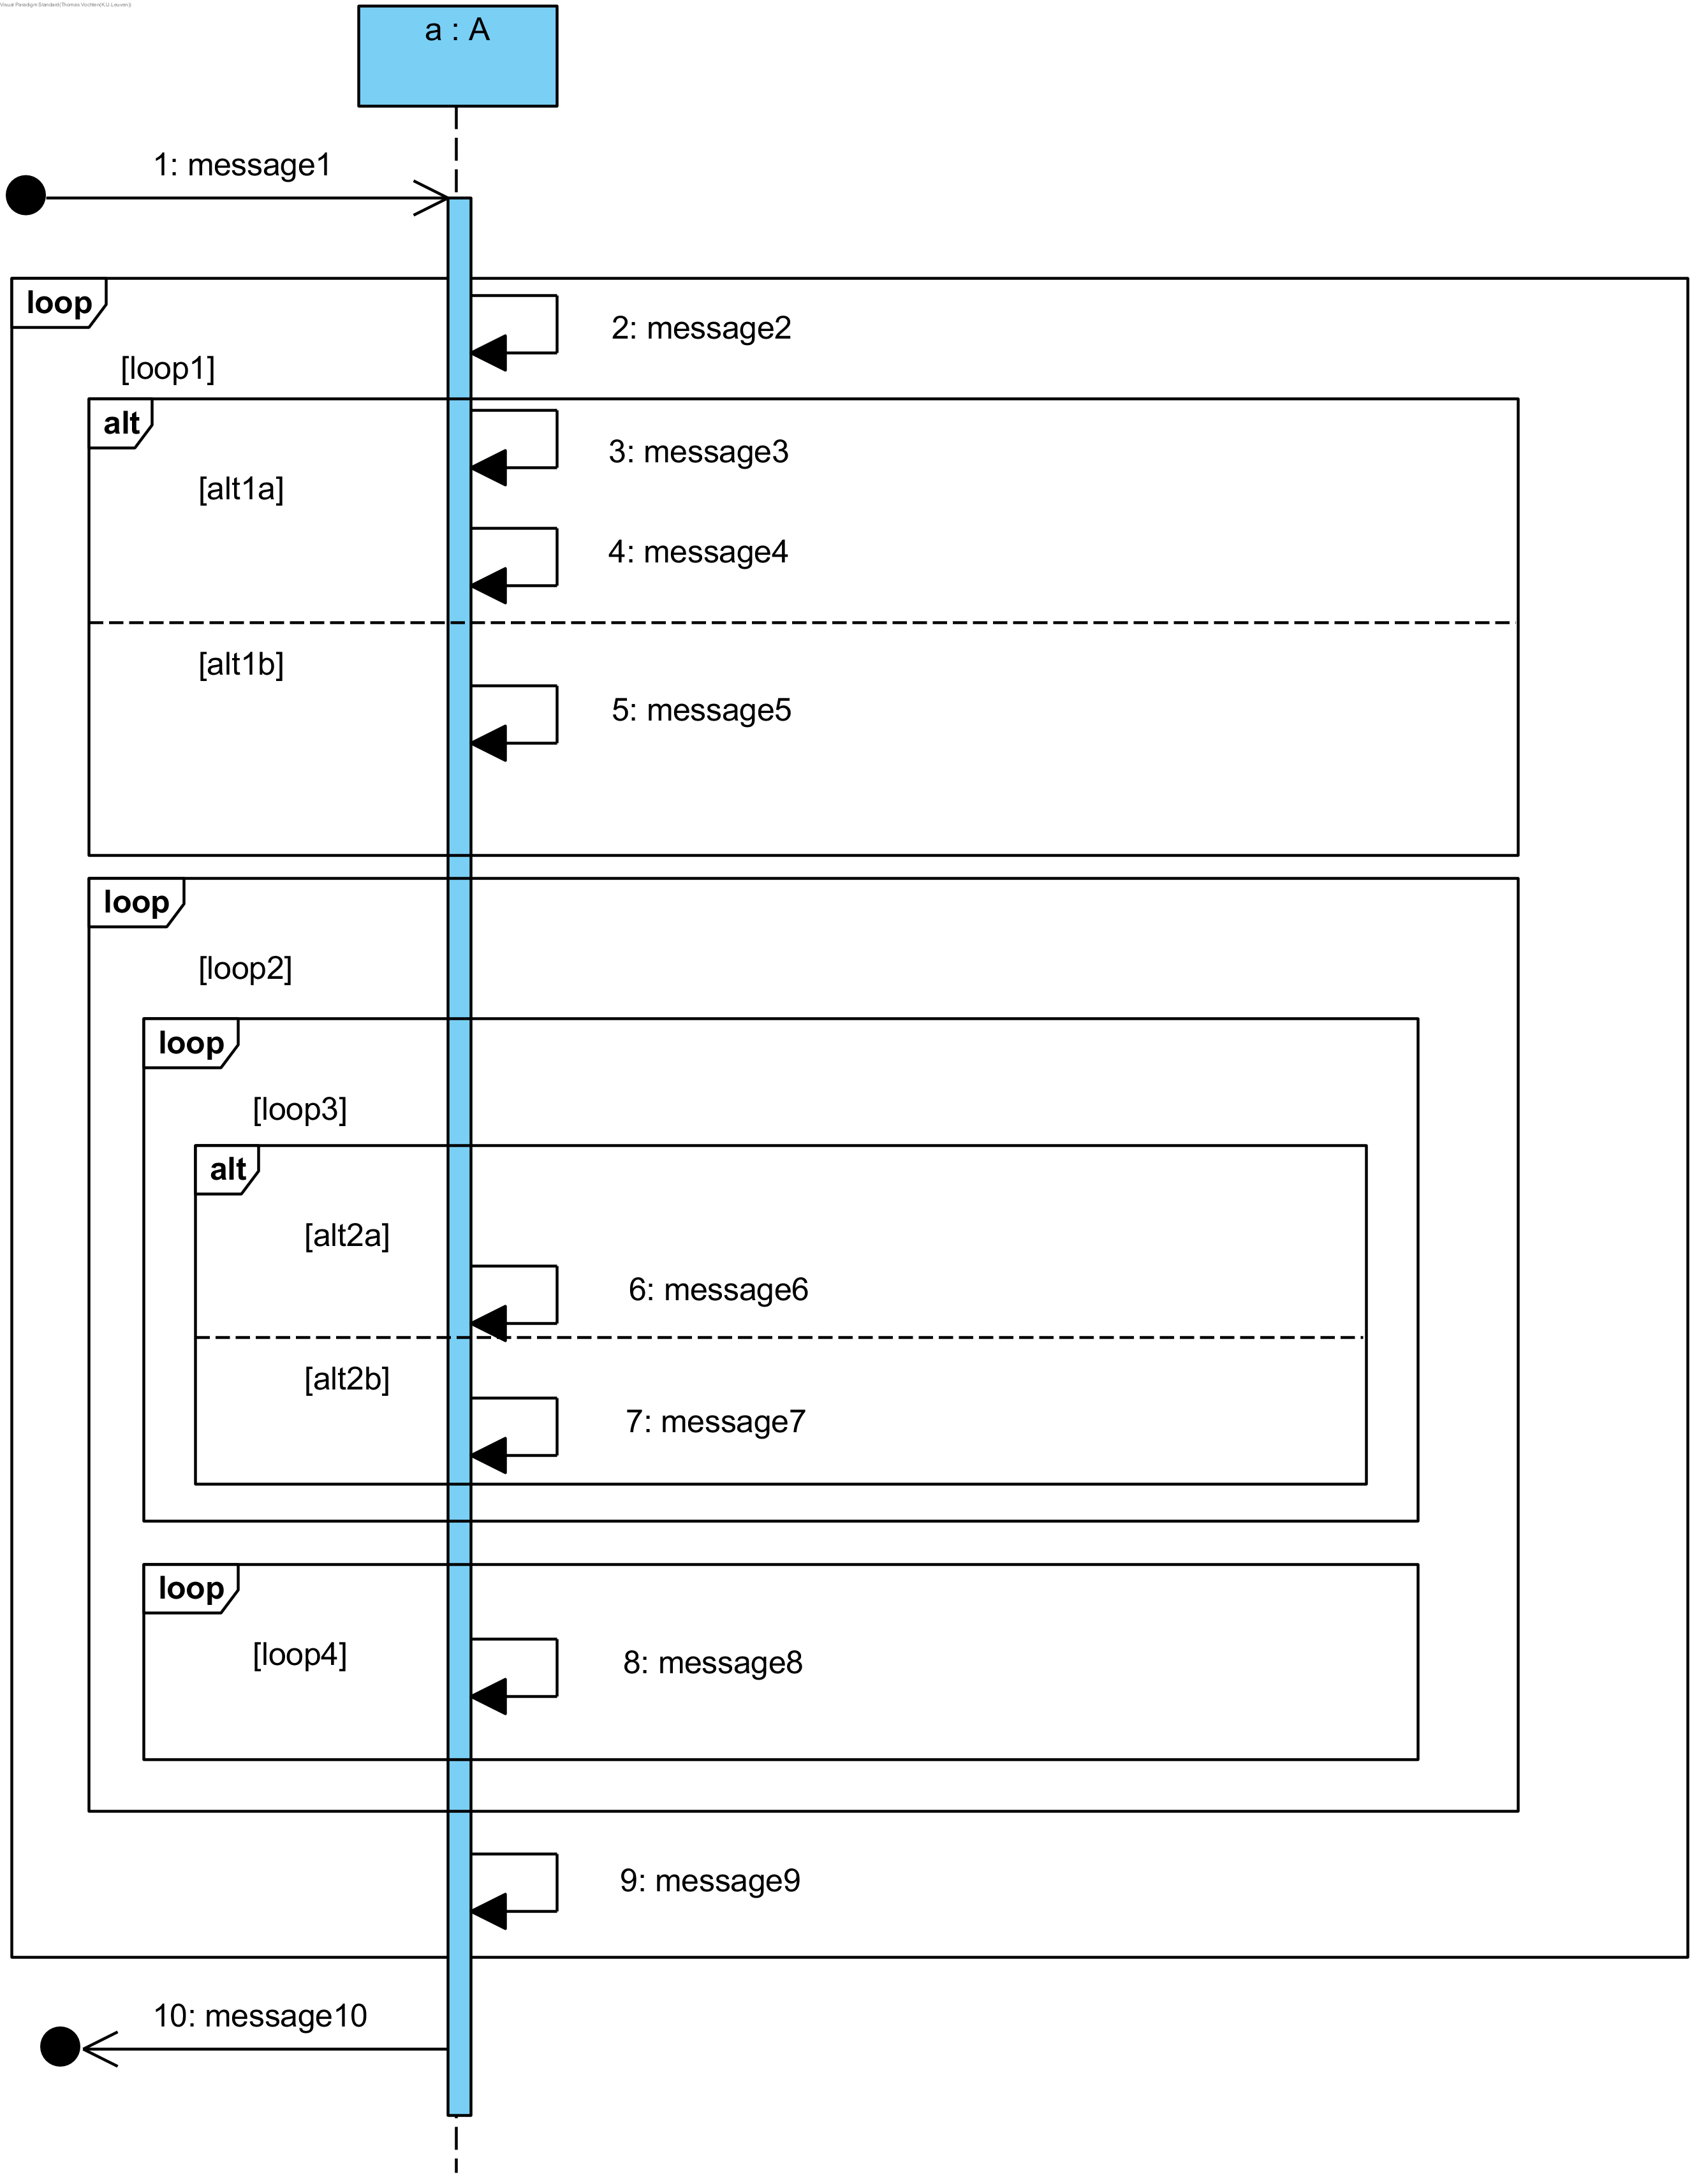
\includegraphics[width=1\textwidth]{chap-gedrag/seq-diagram-frag-ex.png}
	\caption{Sequentiediagram voor een voorbeeldvertaling van gecombineerde fragmenten}
	\label{fig:seq-diagram-frag-ex}
\end{figure}

In wat volgt gebruiken we de voorwaarde voor een fragment als naam voor het fragment zelf. Om het onderscheid te maken tussen deze twee manieren waarop we de voorwaarde gebruiken, schrijven we \fragname{loop1} om aan te duiden dat de voorwaarde als naam wordt gebruikt en \fragcond{loop1} wanneer we het effectief als voorwaarde voor de uitvoering van een fragment gebruiken. \fragname{alt1} verwijst naar het gehele alt-fragment en \fragname{alt1a} en \fragname{alt1b} verwijzen respectievelijk naar het \textit{if}-deel en het \textit{else}-deel.

We roepen algoritme \ref{alg:processCombinedFragment} eerst op op met \fragname{loop1} als argument. Aangezien het geen ouder heeft en \fragmessage{message1}, wat geen fragment heeft, eraan voorafgaat, noteren we in de uitvoer:

\begin{align*}
	&\transitionentry[\fragmessage{message1}]{\lnot \fragcond{loop1}}{\fragmessage{message10}}
\end{align*}

Er is geen fragment dat v\'o\'or dit fragment komt, dus roepen we algoritme \ref{alg:transition-to-frag} op. \fragmessage{message2} is rechtstreeks deel van \fragname{loop1}, dus noteren we in de uitvoer voor dit algoritme:

\begin{align*}
	\transitionentry{\fragcond{loop1}}{\fragmessage{message2}}
\end{align*}

Hierna gaan we verder naar algoritme \ref{alg:wrap-loops} met \fragname{alt1} en \fragname{loop2} als invoerfragmenten en \textit{allemaal} gezet naar \textbf{true}. \fragname{alt1} is geen lusfragment en slaan we over. Vervolgens roepen we algoritme \ref{alg:transition-to-frag} op met \fragname{loop2} als argument.
\fragmessage{message6} is niet rechtstreeks deel van \fragname{loop2}, dus zetten we \textit{voorwaarde} naar \fragcondt{loop2} en roepen eerst algoritme \ref{alg:transition-to-frag} op met \fragname{loop3} als argument. Op dit niveau wordt \textit{voorwaarde} gezet naar ``\fragcond{loop2} $\land$ \fragcond{loop3}'' en roepen we algoritme \ref{alg:transition-to-frag} op met \fragname{alt2} als argument. \fragmessage{message6} en \fragmessage{message7} zijn rechtstreeks deel van \fragname{alt2}, dus hebben we:

\begin{align*}
	&\transitionentry{\fragcond{loop2} \land \fragcond{loop3} \land \fragcond{alt2a}}{\fragmessage{message6}} \\
	&\transitionentry{\fragcond{loop2} \land \fragcond{loop3} \land \fragcond{alt2b}}{\fragmessage{message7}}
\end{align*}

We keren terug naar het niveau van \fragname{loop2}. \fragname{loop3} was een lus, dus zetten we \textit{voorwaarde} naar ``\fragcond{loop2} $\land \lnot$ \fragcond{loop3}'' en roepen we algoritme \ref{alg:wrap-loops} op met als argument de verzameling met enkel \fragname{loop4} als lid. Het resultaat van die oproep is dat we neerschrijven:

\begin{align*}
	\transitionentry{\fragcond{loop2} \land \lnot \fragcond{loop3} \land \fragcond{loop4}}{\fragmessage{message8}}
\end{align*}

We keren terug naar het niveau van \fragname{loop2}. Dit fragment heeft verder geen kinderen, dus eindigt deze oproep van algoritme \ref{alg:wrap-loops} hier.

We keren terug naar stap 7 in algoritme \ref{alg:transition-to-frag} voor \fragname{loop1}. \fragname{alt1} is niet eerder gemarkeerd door algoritme \ref{alg:wrap-loops}, dus gebruiken we het als argument voor een oproep van algoritme \ref{alg:transition-to-frag}. Het resultaat van die oproep is:

\begin{align*}
	&\transitionentry{\fragcond{alt1a}}{\fragmessage{message3}} \\
	&\transitionentry{\fragcond{alt1b}}{\fragmessage{message5}}
\end{align*}

Dit markeert het einde van algoritme \ref{alg:transition-to-frag} voor \fragname{loop1}. In algoritme \ref{alg:processCombinedFragment} gaan we nu over naar stap 10. Na het uitvoeren van de lus verkrijgen we:

\begin{align*}
	&\transitionentry[\fragmessage{message1}]{\fragcond{loop1}}{\fragmessage{message2}} \\
	&\transitionentry[\fragmessage{message2}]{\fragcond{alt1a}}{\fragmessage{message3}} \\
	&\transitionentry[\fragmessage{message2}]{\fragcond{alt1b}}{\fragmessage{message5}} \\
	&\transitionentry[\fragmessage{message4}]{\fragcond{loop2} \land \fragcond{loop3} \land \fragcond{alt2a}}{\fragmessage{message6}} \\
	&\transitionentry[\fragmessage{message5}]{\fragcond{loop2} \land \fragcond{loop3} \land \fragcond{alt2a}}{\fragmessage{message6}} \\
	&\transitionentry[\fragmessage{message4}]{\fragcond{loop2} \land \fragcond{loop3} \land \fragcond{alt2b}}{message7} \\
	&\transitionentry[\fragmessage{message5}]{\fragcond{loop2} \land \fragcond{loop3} \land \fragcond{alt2b}}{message7} \\
	&\transitionentry[\fragmessage{message6}]{\fragcond{loop2} \land \lnot \fragcond{loop3} \land \fragcond{loop4}}{message8} \\
	&\transitionentry[\fragmessage{message7}]{\fragcond{loop2} \land \lnot \fragcond{loop3} \land \fragcond{loop4}}{message8}
\end{align*}

Nu bereiken we stap 18 in algoritme \ref{alg:processCombinedFragment}. Deze stap houdt in dat we algoritme \ref{alg:calcExitForMessages} oproepen met \fragname{loop1} als argument.

In stap 1 roepen we eerst algoritme \ref{alg:determineFinalMessage} op met \fragname{loop1} als argument. De uitkomst daarvan is dat \fragmessage{message9} herkend wordt als laatste bericht. \fragname{loop1} heeft geen ouder, dus gebruiken we algoritme \ref{alg:exitToOutside} met \fragname{loop1} als fragment en ``$\lnot$ \fragcond{loop1}'' als transitievoorwaarde als invoer. Er volgen geen fragmenten op \fragname{loop1} en \fragmessage{message10} is geen deel van een fragment, dus noteren we:

\begin{align*}
	\transitionentry{\lnot \fragcond{loop1}}{\fragmessage{message10}}
\end{align*}

Voor stap 6 in algoritme \ref{alg:calcExitForMessages} noteren we:

\begin{align*}
	\transitionentry[\fragmessage{message9}]{\lnot \fragcond{loop1}}{\fragmessage{message10}}
\end{align*}

Algoritme \ref{alg:calcExitForMessages} gaat nu verder met de kinderen van \fragname{loop1}. \fragname{alt1} komt eerst aan bod, en we bekijken eerst het \textit{if}-deel. Het resultaat van algoritme \ref{alg:determineFinalMessage} is \textit{\{\fragmessage{message4}, $\epsilon$\}}. \fragname{loop1} is de ouder van \fragname{alt1} en \fragmessage{message6} is deel van \fragname{loop1}, dus we gaan naar stap 11. In wat volgt roepen we algoritme \ref{alg:transition-to-frag} op met \fragname{loop2} als argument. Het resultaat daarvan gebruiken we om te noteren:

\begin{align*}
	&\transitionentry[\fragmessage{message4}]{\fragcond{loop2} \land \fragcond{loop3} \land \fragcond{alt2a}}{\fragmessage{message6}} \\
	&\transitionentry[\fragmessage{message4}]{\fragcond{loop2} \land \fragcond{loop3} \land \fragcond{alt2b}}{\fragmessage{message7}} \\
	&\transitionentry[\fragmessage{message4}]{\fragcond{loop2} \land \lnot \fragcond{loop3} \land \fragcond{loop4}}{\fragmessage{message8}}
\end{align*}

Als gevolg van het feit dat \fragmessage{message9} volgt op \fragname{loop2}, noteren we ook:

\begin{align*}
	&\transitionentry[\fragmessage{message4}]{\lnot \fragcond{loop2}}{message9}
\end{align*}

Het voorgaande wordt herhaald voor het \textit{else}-deel. Op gelijkaardige wijze voor het \textit{if}-deel leidt dit tot:

\begin{align*}
	&\transitionentry[\fragmessage{message5}]{\fragcond{loop2} \land \fragcond{loop3} \land \fragcond{alt2a}}{\fragmessage{message6}} \\
	&\transitionentry[\fragmessage{message5}]{\fragcond{loop2} \land \fragcond{loop3} \land \fragcond{alt2b}}{\fragmessage{message7}} \\
	&\transitionentry[\fragmessage{message5}]{\fragcond{loop2} \land \lnot \fragcond{loop3} \land \fragcond{loop4}}{\fragmessage{message8}} \\
	&\transitionentry[\fragmessage{message5}]{\lnot \fragcond{loop2}}{message9}
\end{align*}

We gaan terug naar stap 31 voor \fragname{loop1}. Algoritme \ref{alg:calcExitForMessages} wordt nu opgeroepen op \fragname{loop2}. Via algoritme \ref{alg:determineFinalMessage} concluderen we dat \fragname{loop2} geen laatste bericht heeft, dus roepen we algoritme \ref{alg:calcExitForMessages} op met elk kind om de beurt als argument. \fragname{loop3} komt eerst. Op gelijkaardige wijze gaan we verder naar \fragname{alt2}.

Het \textit{if}-deel van \fragname{alt2} komt eerst. Algoritme \ref{alg:determineFinalMessage} besluit dat \fragmessage{message6} het laatste bericht is. \fragmessage{message8} is geen deel van \fragname{loop3}, dus zetten we \textit{aggregateVoorwaarde} naar ``$\lnot$ \fragcond{loop3}'' en \textit{fragment} naar \fragname{loop2} en gaan naar stap 10. \fragname{message8} is deel van \fragname{loop2}, dus roepen we algoritme \ref{alg:transition-to-frag} op met \fragname{loop4} als argument en concateneren \textit{aggregateVoorwaarde}, wat resulteert in:

\begin{align*}
	\transitionentry[\fragmessage{message6}]{\fragcond{loop4} \land \lnot \fragcond{loop3}}{\fragmessage{message8}}
\end{align*}

\fragname{loop4} is een lus, dus zetten we \textit{fragment} naar \fragname{loop1} en gaan naar stap 10. \fragmessage{message8} is deel van \fragname{loop1}, maar \fragname{loop2} is gemarkeerd in de vorige iteratie en slaan we dus over. We zien wel dat \fragname{loop1} een bericht heeft na \fragmessage{message8}, namelijk \fragmessage{message9}, en daarom noteren we:

\begin{align*}
	\transitionentry[\fragmessage{message6}]{\lnot \fragcond{loop3} \land \lnot \fragcond{loop4} \land \lnot \fragcond{loop2}}{\fragmessage{message9}}
\end{align*}

Met het vinden van dat bericht na \fragmessage{message8}, eindigt het algoritme voor het \textit{if}-deel van \fragname{alt2}. Nu komt het \textit{else}-deel van \fragname{alt2} aan bod, en gelijkaardig voor het \textit{if}-deel krijgen we:

\begin{align*}
		&\transitionentry[\fragmessage{message7}]{\fragcond{loop4} \land \lnot \fragcond{loop3}}{\fragmessage{message8}} \\
		&\transitionentry[\fragmessage{message7}]{\lnot \fragcond{loop3} \land \lnot \fragcond{loop4} \land \lnot \fragcond{loop2}}{\fragmessage{message9}}
\end{align*}

\fragname{loop3} is nu volledig behandeld, en we gaan terug naar stap 31 voor \fragname{loop2}. We roepen algoritme \ref{alg:calcExitForMessages} op met \fragname{loop4} als argument. Algoritme \ref{alg:determineFinalMessage} besluit dat \fragmessage{message8} het laatste bericht is en we zetten \textit{aggregateVoorwaarde} naar ``$\lnot$ \fragcond{loop4}''. \fragname{loop2} heeft geen bericht na \fragmessage{message8}, dus zetten we fragment naar \fragname{loop1} en gaan terug naar stap 8. \fragmessage{message9} komt in \fragname{loop1} meteen na \fragmessage{message8} en is rechtstreeks deels van \fragname{loop1}, dus noteren we:

\begin{align*}
	\transitionentry[\fragmessage{message8}]{\lnot \fragcond{loop4} \land \lnot \fragcond{loop2}}{\fragmessage{message9}}
\end{align*}

Hier stopt de uitvoering van het algoritme voor \fragname{loop4}, en hiermee meteen ook voor \fragname{loop2} en \fragname{loop1}.

\parbreak

We bereiken stap 19 in algoritme \ref{alg:processCombinedFragment}. In plaats van \fragname{loop1} te gebruiken als argument zoals het zou zijn in een echte uitvoering, gebruiken we \fragname{loop4} als illustratiever voorbeeld.

\fragmessage{message8} is vanzelfsprekend het laatste bericht van \fragname{loop4}. We roepen de variant van algoritme \ref{alg:transition-to-frag} gebruikt in dit algoritme op met \fragname{loop4} als argument. De uitkomst van deze iteratie is:

\begin{align*}
	\transitionentry[\fragmessage{message8}]{\fragcond{loop4}}{\fragmessage{message8}}
\end{align*}

We voegen \fragname{loop4} toe aan \textit{uitgesloten} en zetten \textit{aggregateVoorwaarde} naar ``$\lnot$ \fragcond{loop4}'' en \textit{fragment} naar \fragname{loop2}. De laatste container van \fragname{loop2} is een fragment en \fragmessage{message8} is daar het laatste bericht van, dus zetten we \textit{bundelVoorwaarde} naar ``\fragcond{loop2}''. \fragname{loop4} is lid van \textit{uitgesloten}, dus noteren we:

\begin{align*}
	&\transitionentry[\fragmessage{message8}]{\lnot \fragcond{loop4} \land \fragcond{loop2} \land \fragcond{loop3} \land \fragcond{alt2a}}{\fragmessage{message6}} \\
	&\transitionentry[\fragmessage{message8}]{\lnot \fragcond{loop4} \land \fragcond{loop2} \land \fragcond{loop3} \land \fragcond{alt2b}}{\fragmessage{message7}}
\end{align*}

We voegen \fragname{loop2} toe aan \textit{uitgesloten}, concateneren \textit{aggregateVoorwaarde} met ``$\land \lnot$ \fragcond{loop2}'' en gaan verder met \fragname{loop1}. \fragmessage{message8} is geen laatste bericht van \fragname{loop1}, en \fragname{loop1} heeft geen ouder. De uitvoering van algoritme \ref{alg:calculateLoopReentry} stopt.

\parbreak

Nadat we algoritme \ref{alg:processCombinedFragment} hebben uitgevoerd op alle fragmenten, rest de taak van de uitvoer van dat algoritme te vertalen naar logica.

\subsubsection{De uitvoer van de algoritmes vertalen naar logica}

Het is eenvoudig om de uitvoer te vertalen naar logica. We zoeken naar gevallen waar het bericht waarnaar gesprongen wordt en de voorwaarde waaronder die sprong gebeurt overeenkomen en combineren ze. Als voorbeeld:

\begin{align*}
	&\transitionentry[\fragmessage{$message_b$}]{\fragcond{voorwaarde}}{\fragmessage{$message_a$}} \\
	&\transitionentry[\fragmessage{$message_c$}]{\fragcond{voorwaarde}}{\fragmessage{$message_a$}}
\end{align*}

Dit vertalen we naar:

\begin{align*}
	\forall{t}[Time](C\_SDPointAt(Next(t), message_a) \leftarrow (SDPointAt(t, message_b) \\ \lor SDPointAt(t, message_c)) \land \fragcond{voorwaarde}).
\end{align*}

De uitvoer van algoritme \ref{alg:processCombinedFragment} voor alle fragmenten in figuur \ref{fig:seq-diagram-frag-ex} vertalen we op die manier als volgt naar logica:

\begin{align*}
	&\forall{t}[Time](C\_SDPointAt(Next(t), 2) \leftarrow (SDPointAt(t, 1) \\ &\lor SDPointAt(t, 9)) \land \fragcond{loop1}). \\
	&\forall{t}[Time](C\_SDPointAt(Next(t), 3) \leftarrow SDPointAt(t, 2) \\ &\land \fragcond{alt1a}). \\
	&\forall{t}[Time](C\_SDPointAt(Next(t), 5) \leftarrow SDPointAt(t, 2) \\ &\land \fragcond{alt1b}). \\
	&\forall{t}[Time](C\_SDPointAt(Next(t), 6) \leftarrow (SDPointAt(t, 6) \\ &\lor SDPointAt(t, 7)) \land \fragcond{loop3} \land \fragcond{alt2a})). \\
	&\forall{t}[Time](C\_SDPointAt(Next(t), 6) \leftarrow SDPointAt(t, 8) \\ &\land \lnot \fragcond{loop4} \land \fragcond{loop2} \land \fragcond{loop3} \land \fragcond{alt2a}). \\
	&\forall{t}[Time](C\_SDPointAt(Next(t), 6) \leftarrow (SDPointAt(t, 4) \\ &\lor SDPointAt(t, 5)) \land \fragcond{loop2} \land \fragcond{loop3} \land \fragcond{alt2a}). \\
	&\forall{t}[Time](C\_SDPointAt(Next(t), 7) \leftarrow (SDPointAt(t, 6) \\ &\lor SDPointAt(t, 7)) \land \fragcond{loop3} \land \fragcond{alt2b})). \\
	&\forall{t}[Time](C\_SDPointAt(Next(t), 7) \leftarrow SDPointAt(t, 8) \\ &\land \lnot \fragcond{loop4} \land \fragcond{loop2} \land \fragcond{loop3} \land \fragcond{alt2b}). \\
	&\forall{t}[Time](C\_SDPointAt(Next(t), 7) \leftarrow (SDPointAt(t, 4) \\ &\lor SDPointAt(t, 5)) \land \fragcond{loop2} \land \fragcond{loop3} \land \fragcond{alt2b}).
\end{align*}

\begin{align*}
	&\forall{t}[Time](C\_SDPointAt(Next(t), 8) \leftarrow (SDPointAt(t, 6) \\ &\lor SDPointAt(t, 7)) \land \lnot \fragcond{loop3} \land \fragcond{loop4}). \\
	&\forall{t}[Time](C\_SDPointAt(Next(t), 8) \leftarrow (SDPointAt(t, 4) \\ &\lor SDPointAt(t, 5)) \land \fragcond{loop2} \land \lnot \fragcond{loop3} \\ &\land \fragcond{loop4}). \\
	&\forall{t}[Time](C\_SDPointAt(Next(t), 8) \leftarrow SDPointAt(t, 8) \\ &\land \fragcond{loop4}). \\
	&\forall{t}[Time](C\_SDPointAt(Next(t), 9) \leftarrow (SDPointAt(t, 6) \\ &\lor SDPointAt(t, 7)) \land \lnot \fragcond{loop3} \land \lnot \fragcond{loop4} \\ &\land \lnot \fragcond{loop2}). \\
	&\forall{t}[Time](C\_SDPointAt(Next(t), 9) \leftarrow SDPointAt(t, 8) \\ &\land \lnot \fragcond{loop4} \land \lnot \fragcond{loop2}). \\
	&\forall{t}[Time](C\_SDPointAt(Next(t), 9) \leftarrow (SDPointAt(t, 4) \\ &\lor SDPointAt(t, 5)) \land \lnot \fragcond{loop2}). \\
	&\forall{t}[Time](C\_SDPointAt(Next(t), 10) \leftarrow (SDPointAt(t, 1) \\ &\lor SDPointAt(t, 9)) \land \lnot \fragcond{loop1}).
\end{align*}

\section{Interactie tussen meerdere sequentiediagrammen}\label{sec:interaction}
In een project stelt men doorgaans meerdere sequentiediagrammen op die elkaar ook kunnen oproepen. Men gebruikt soms ook recursie in deze diagrammen. Deze sectie beschrijft hoe we het oproepen van andere sequentiediagrammen en een recursiemechanisme ondersteunen.

\begin{figure}
	\centering
	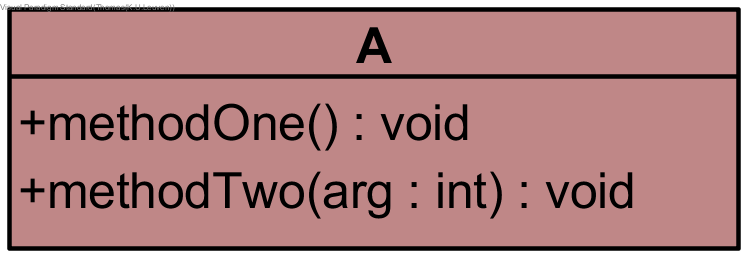
\includegraphics[width=0.25\textwidth]{chap-gedrag/recursion-class.png}
	\caption{Klasse gebruikt in voorbeeld over recursie}
	\label{fig:recursion-class}
\end{figure}

%\begin{landscape}
%\thispagestyle{empty}
%	\begin{sidewaysfigure}[htp]
%		\centering
%		\begin{subfigure}{\textwidth}
%			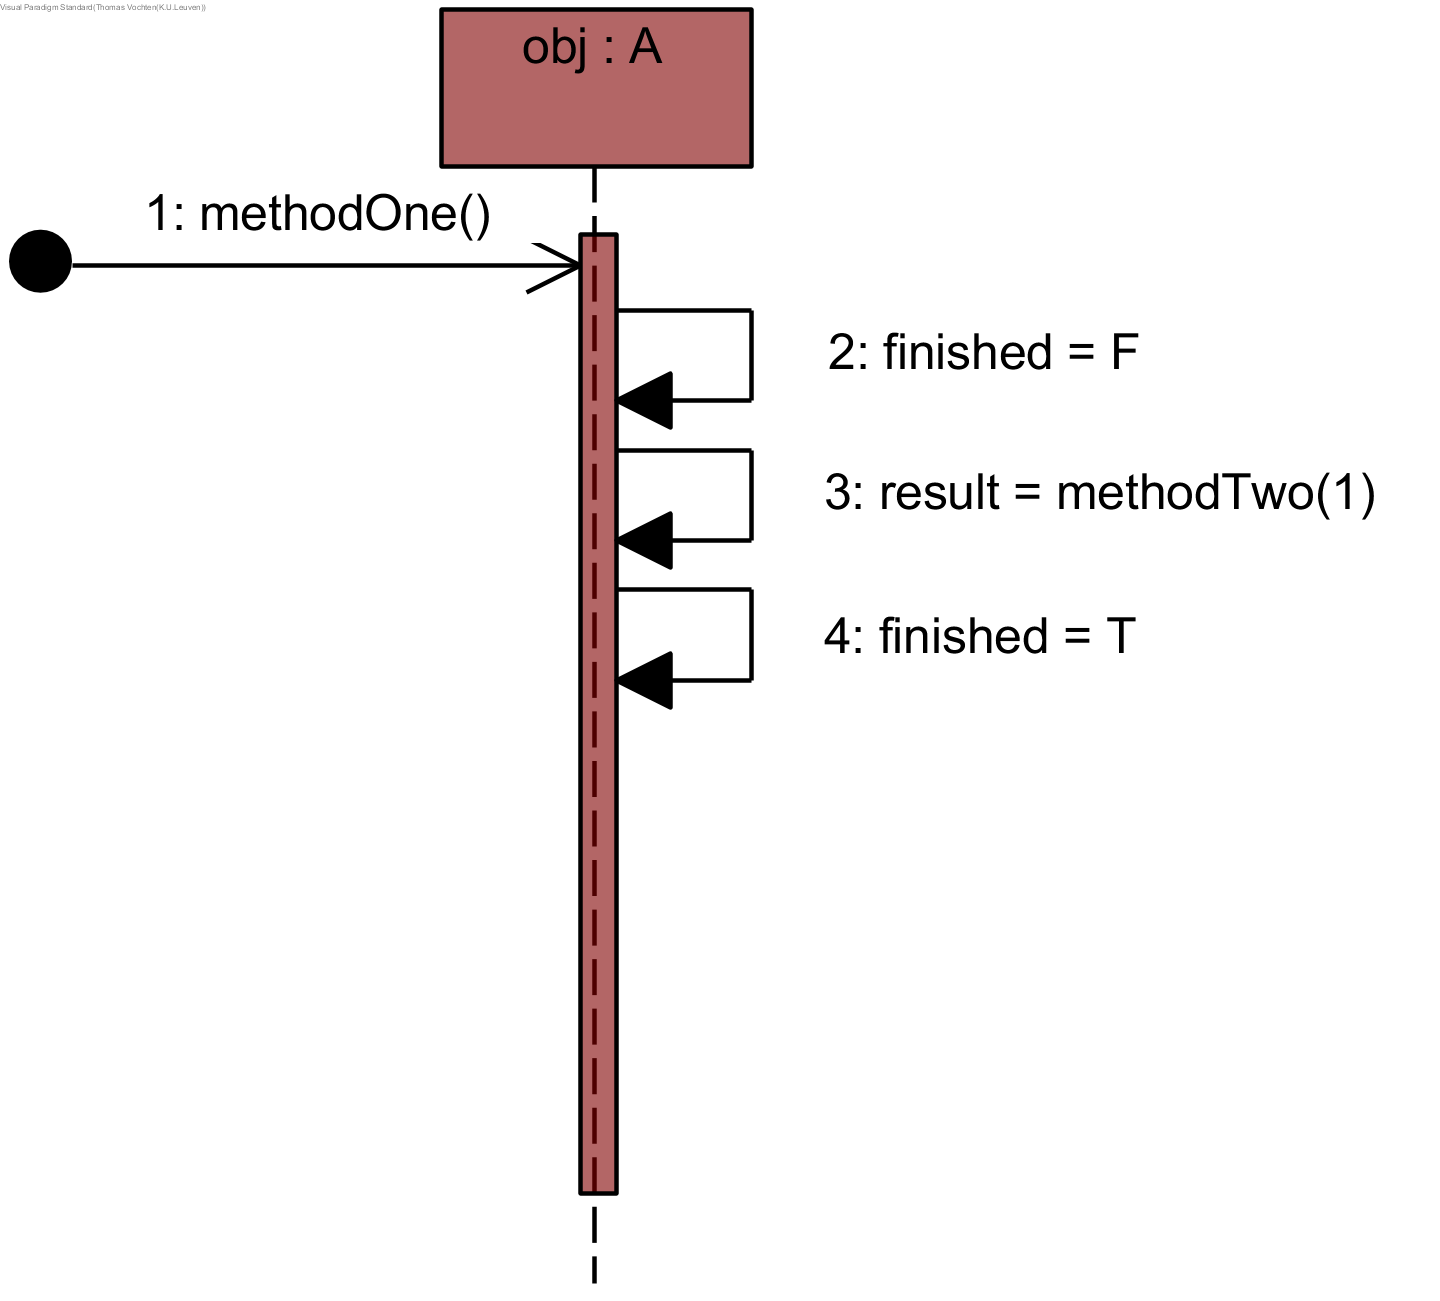
\includegraphics[height=0.4\textwidth]{chap-gedrag/methodOne.png}
%			\caption{Sequentiediagram voor methodOne()}
%			\label{fig:methodOne}
%		\end{subfigure}%
%		\begin{subfigure}{\textwidth}
%			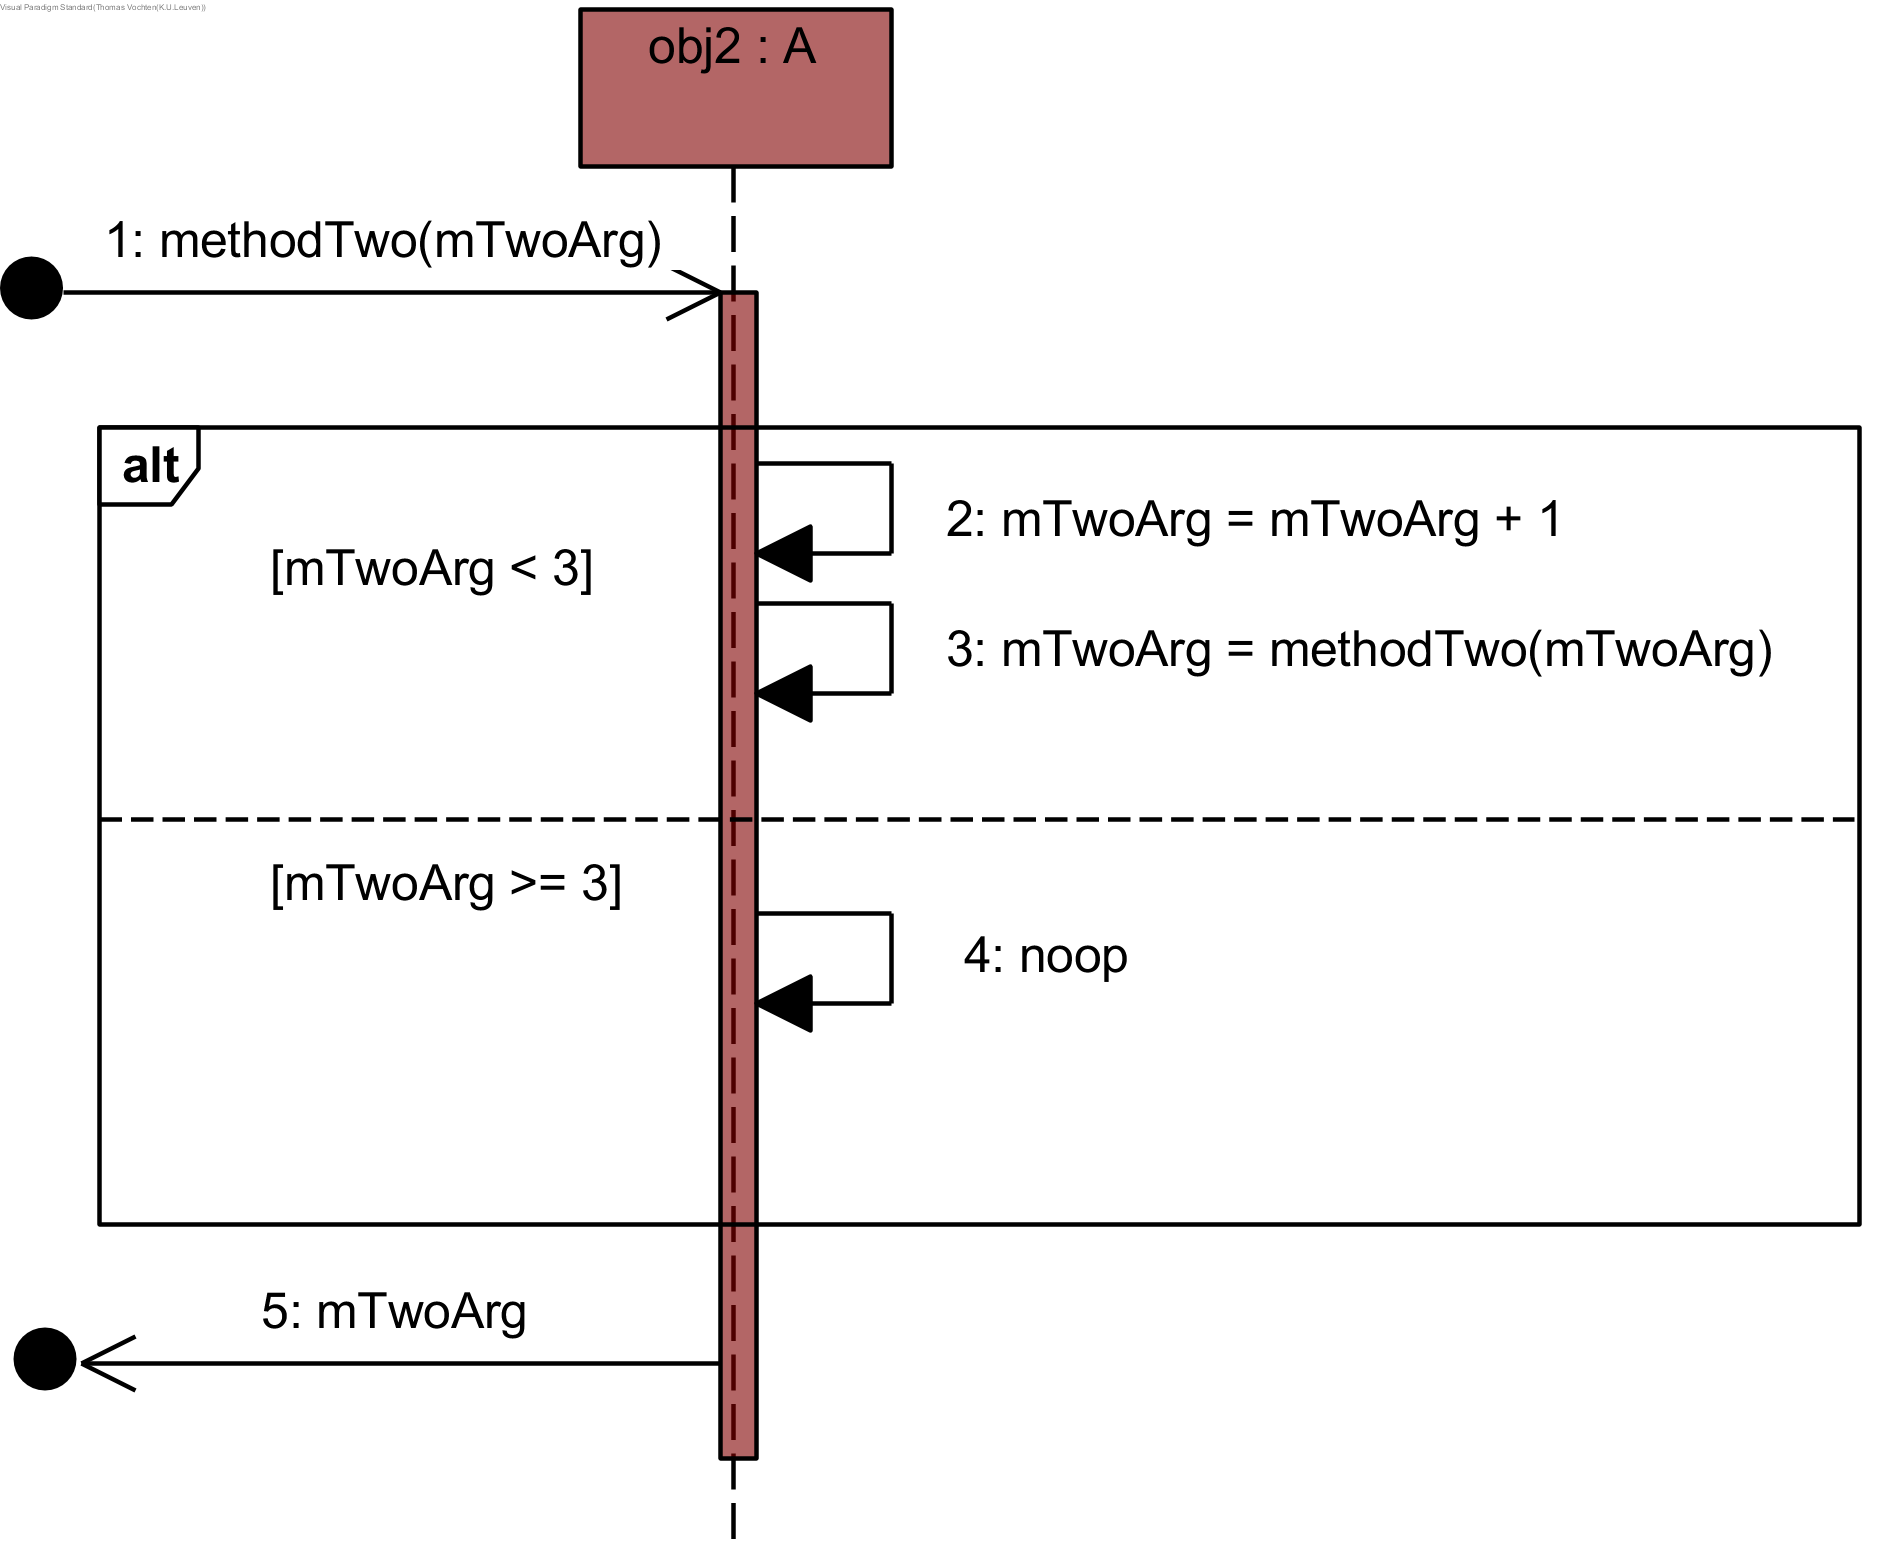
\includegraphics[height=0.4\textwidth]{chap-gedrag/methodTwo.png}
%			\caption{Sequentiediagram voor methodTwo()}
%			\label{fig:methodtwo}
%		\end{subfigure}
%		\caption{Sequentiediagrammen voor klasse A in figuur \ref{fig:recursion-class}}
%		\label{fig:seq-recursion}
%	\end{sidewaysfigure}
%\end{landscape}

\begin{figure}[htp]
	\centering
	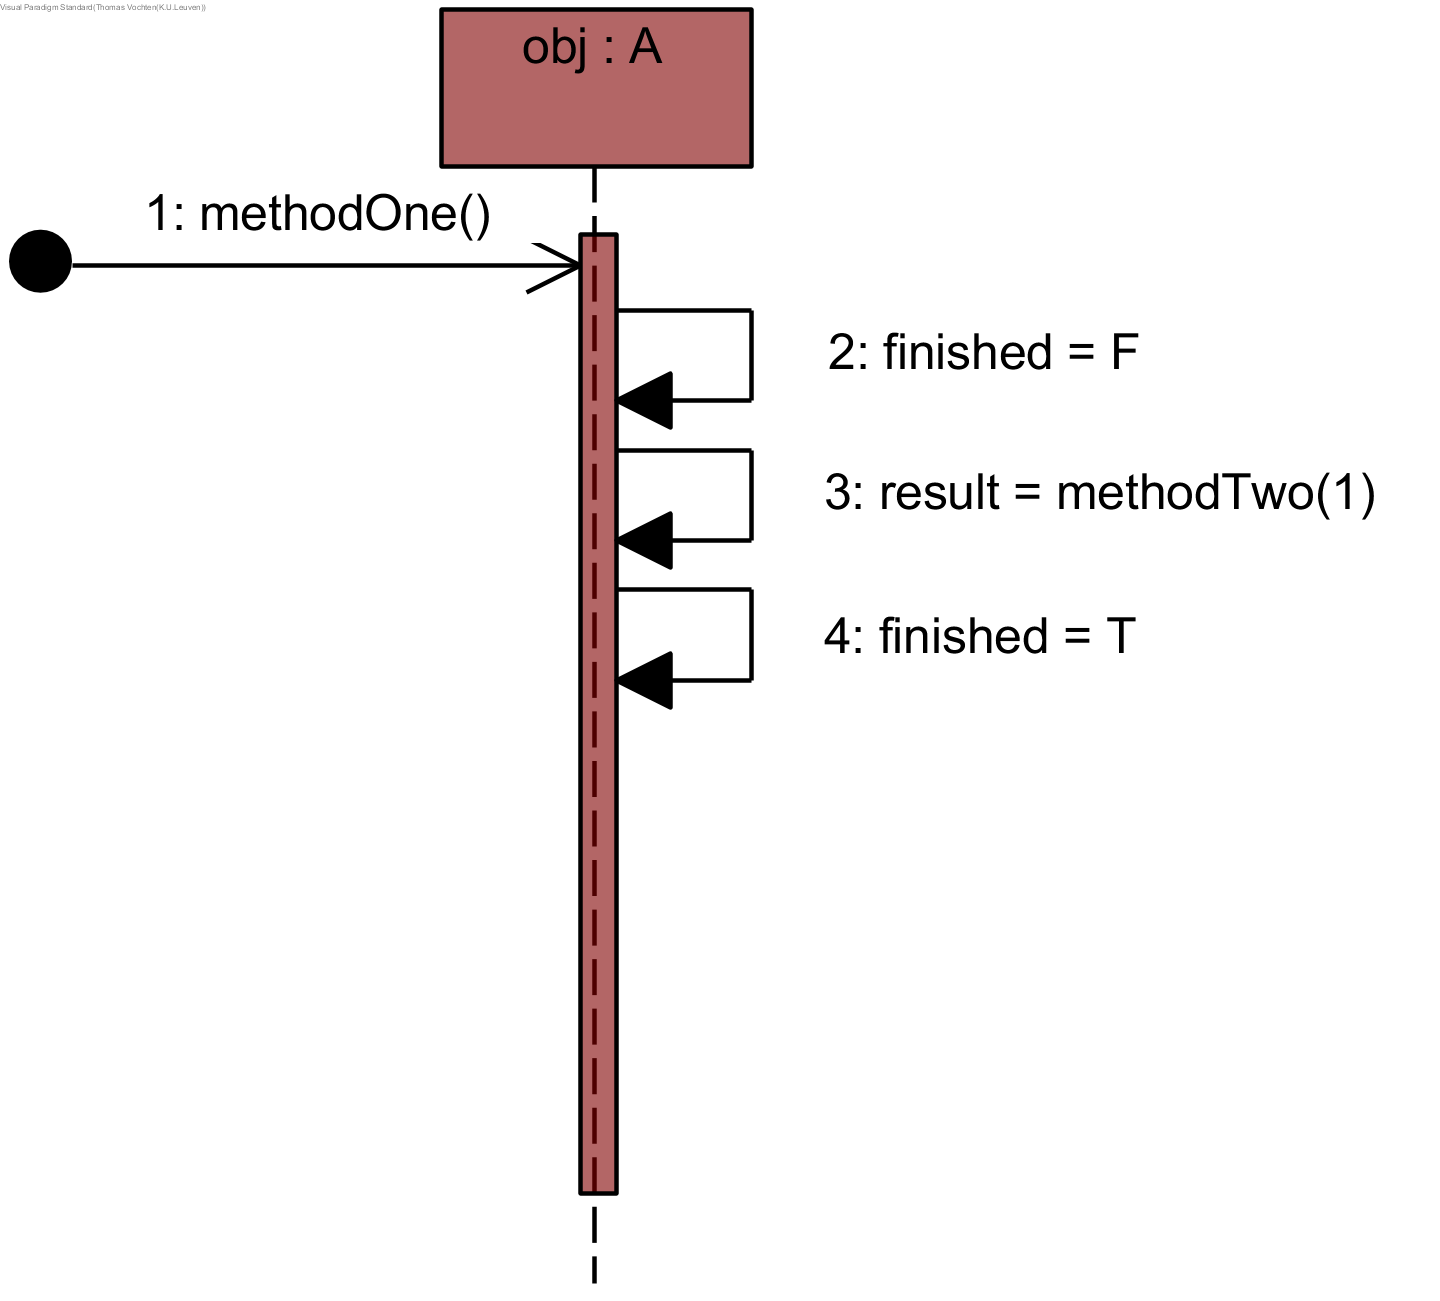
\includegraphics[width=0.5\textwidth]{chap-gedrag/methodOne.png}
	\caption{Sequentiediagram voor methodOne()}
	\label{fig:methodOne}
\end{figure}%

\begin{figure}[htp]
	\centering
	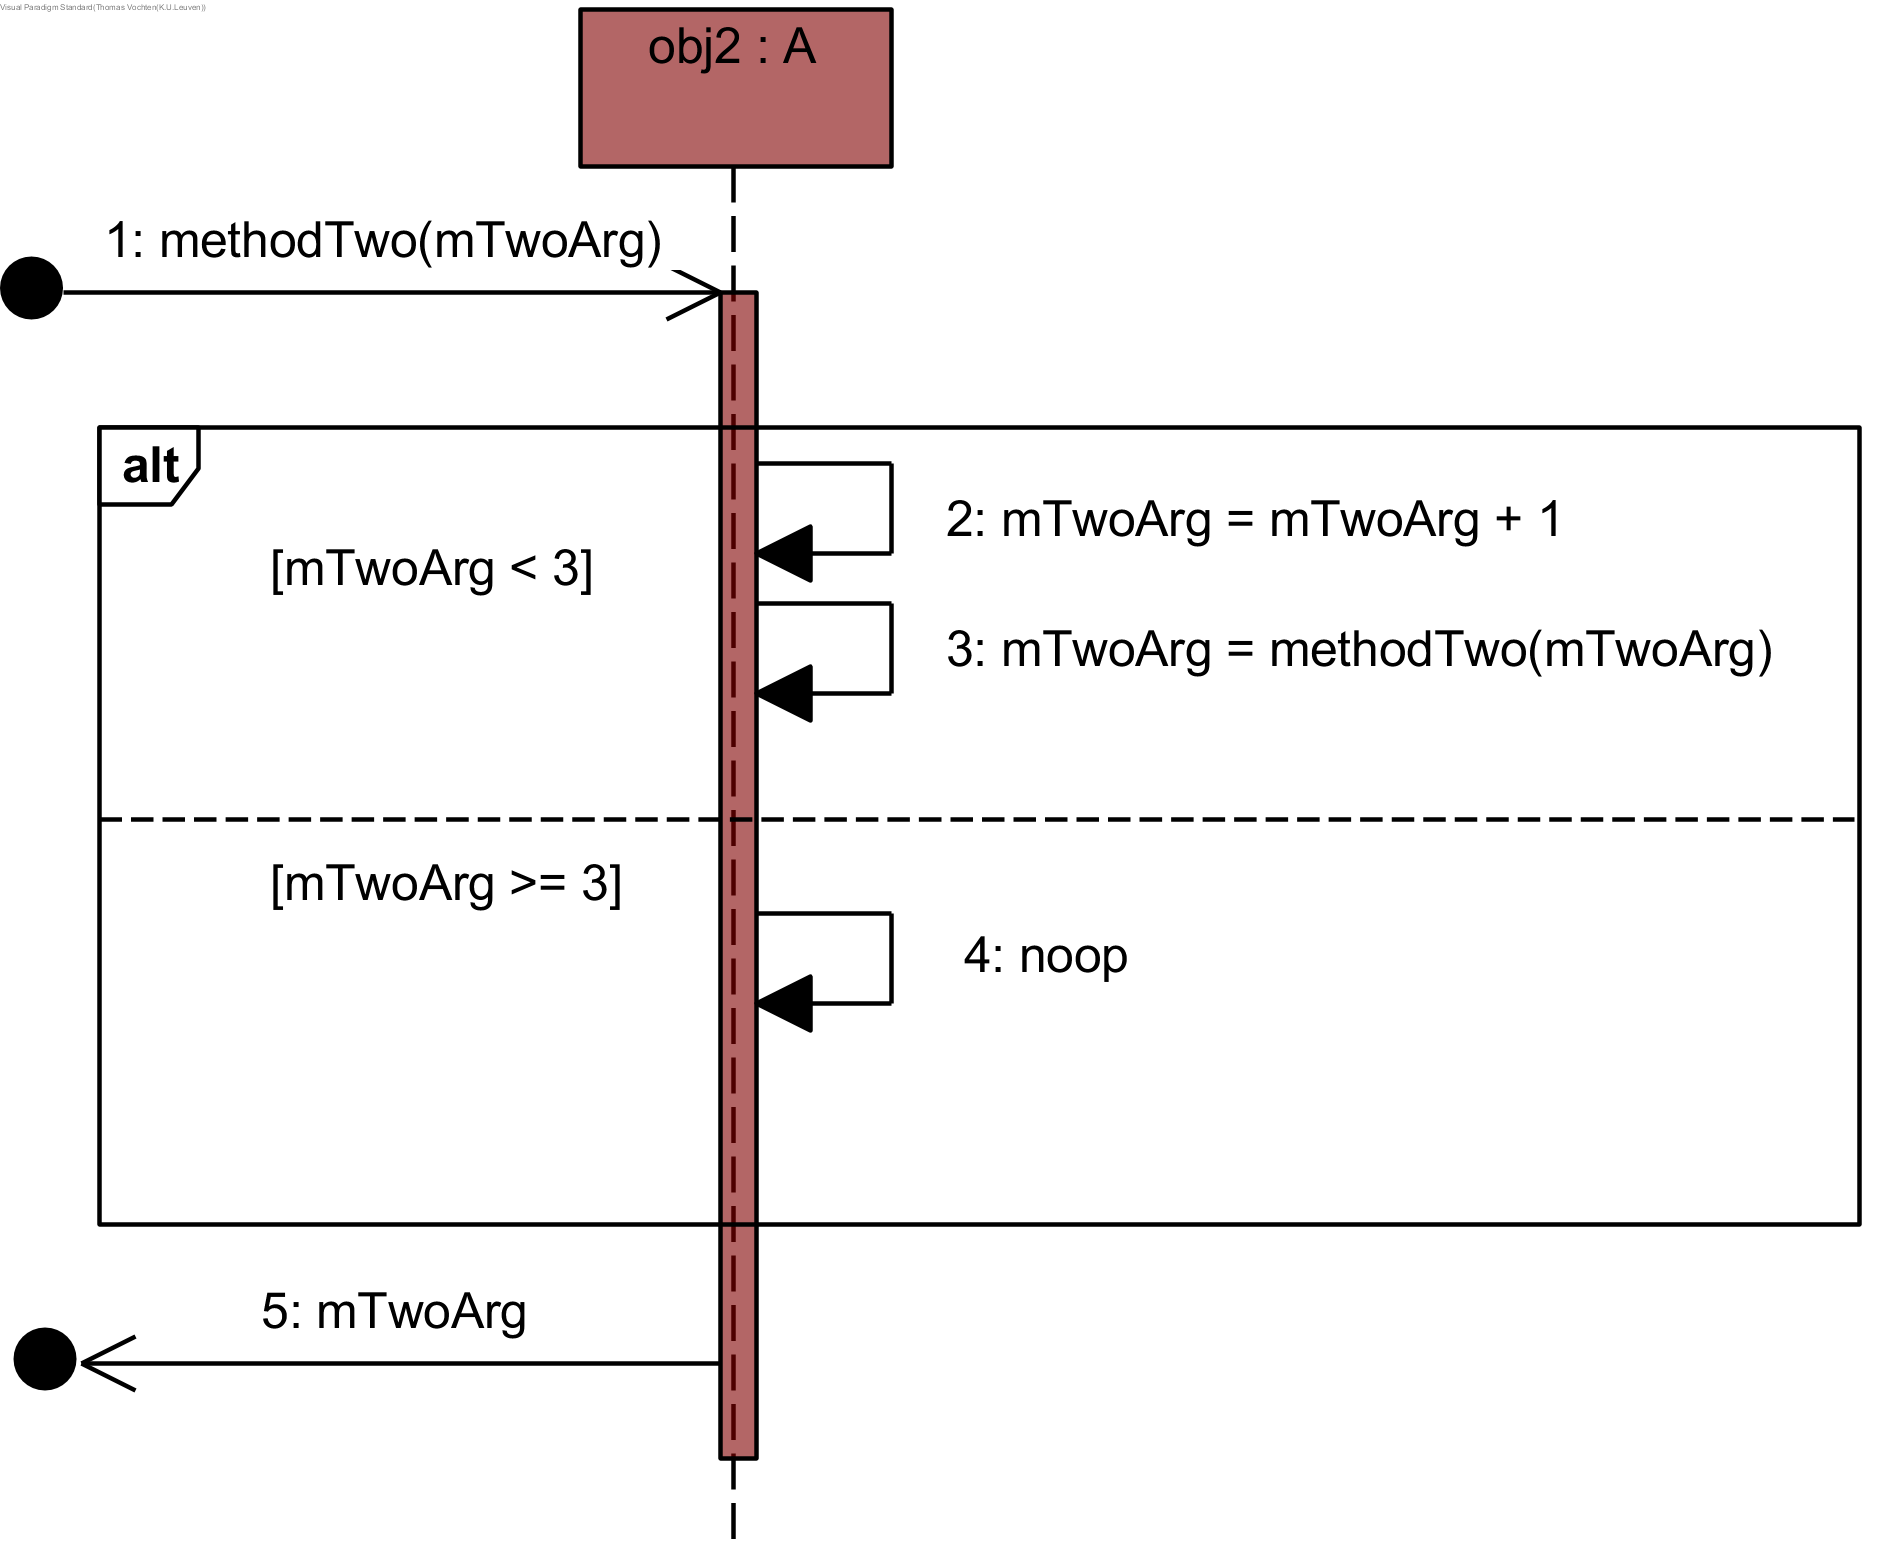
\includegraphics[width=0.7\textwidth]{chap-gedrag/methodTwo.png}
	\caption{Sequentiediagram voor methodTwo()}
	\label{fig:methodtwo}
\end{figure}

In de volgende subsecties gebruiken we het voorbeeld uitgebeeld in figuren \ref{fig:recursion-class}, \ref{fig:methodOne} en \ref{fig:methodtwo} om de gebruikte principes te illustreren.

\subsection{Aanpassingen aan \textit{SDPoint}}
Het is niet meer voldoende om \textit{SDPoint}s te modelleren als natuurlijke getallen aangezien elk diagram zijn eigen \textit{SDPoint}s heeft. Om de \textit{SDPoint}s horende bij elk diagram van elkaar te kunnen onderscheiden, maken we van het logisch type \textit{SDPoint} nu een \textit{constructed type} in IDP. We gebruiken als patroon voor de naamgeving van elk logisch object $<diagramnaam>\_<instructienummer>$. Voor het voorbeeld krijgen we o.a. $methodOne\_2$ en $methodTwo\_3$. We voegen ook een nieuwe functie toe aan het vocabularium dat gegeven een \textit{SDPoint} het volgende \textit{SDPoint} teruggeeft, namelijk $NextSD(SDPoint) : SDPoint$.

Een andere aanpassing is dat we een virtuele \textit{SDPoint} inpassen na elke instructie voor een oproep. Het naamgevingspatroon hiervoor is $<diagramnaam>\_<instructienummer>post$. Aangezien de derde instructie in figuur \ref{fig:methodOne} een oproep is, krijgen we $methodOne\_3post$. Met deze toevoeging ontkoppelen we twee zaken die bij een oproep komen kijken: Enerzijds dat het mogelijk is dat het resultaat van een oproep wordt toegekend aan een variabele; en anderzijds dat na een oproep er mogelijks een alt-fragment of lusfragment volgt, en dat het dus v\'o\'or de oproep niet noodzakelijk duidelijk is welke de volgende instructie is na de uitvoering van de oproep. Het zou niet mogelijk zijn om voor deze twee zaken het correcte gedrag te verkrijgen zonder een oproepinstructie op deze manier op te splitsen.

\subsection{Het stapelmechanisme}
Om oproepen van andere sequentiediagrammen correct uit te voeren, moet de theorie bijhouden welke variabelen er bestaan tijdens een bepaalde oproep. Bovendien moet de theorie voor recursieve oproepen ook de waardes van een set variabelen kunnen bewaren v\'o\'or een oproep en die waardes herstellen na een oproep. Hiertoe ontwerpen we een stapelmechanisme. Er gebeuren volgende aanpassingen aan het vocabularium:

\begin{itemize}
	\item Toevoeging van het logisch type $StackLevel \subset \mathbb{N}$: Dit stelt de oproepdiepte van een oproep voor.
	\item Toevoeging van een inerti\"ele functie $CurrentStackLevel(Time) : StackLevel$: De oproepdiepte op een bepaald tijdstip.
	\item Toevoeging van een intertieel predicaaat \\ $ReturnPoint(Time, StackLevel, SDPoint)$: Op een bepaald tijdstip, de \textit{SDPoint} waarnaar de uitvoering moet terugkeren wanneer de laatste instructie voor de gegeven \textit{StackLevel} bereikt is.
	\item Alle diagramvariabelen worden nu gemodelleerd door een ternair predicaat dat nu ook de oproepdiepte in rekening neemt. Voor het voorbeeld krijgen we dus bijvoorbeeld $FinishedT(Time, StackLevel, bool)$.
\end{itemize}

De volgende subsecties beschrijven hoe we in het definitieblok voor de causatiezinnen dit stapelmechanisme gebruiken.

\subsubsection{Causatiezinnen voor \textit{SDPointAt/2}}\label{sec:sd-rec-cause}
Oproepinstructies betekenen bijkomende uitzonderingen op het normale verloop van \textit{SDPoints} naast deze die voortkomen uit alt-- en lusfragmenten. In dit geval zijn $methodOne\_3$, $methodTwo\_3$, $methodOne\_5$, $methodTwo\_5$ en $finished$ de nieuwe uitzonderingen. $methodOne\_5$ en $methodTwo\_5$ zijn ook \textit{SDPoint}s die niet in het diagram terug te vinden zijn, maar die we zelf toevoegen. Dit zijn impliciete terugkeerinstructies die we toevoegen voor diagrammen die \textit{void} als resultaat hebben. $finished$ is een speciale \textit{SDPoint} die het einde van de uitvoering aanduidt. De zin die het normale verloop van \textit{SDPoint}s regelt wordt dus:

\begin{align}
	& \nonumber \forall{t}[Time]\forall{s}[SDPoint](C\_SDPointAt(Next(t), NextSD(s) \leftarrow \\ \nonumber &SDPointAt(t,s) \land \lnot((s = methodOne\_3) \lor (s = methodOne\_5) \\ \nonumber &\lor (s = methodTwo\_1) \lor (s = methodTwo\_3) \lor (s = methodTwo\_3post) \\ &\lor (methodTwo\_4) \lor (methodTwo\_5) \lor (s = finished)).
\end{align}

De uitzonderingen als resultaat van een oproep worden als volgt gemodelleerd:

\begin{align}
	 \forall{t}[Time](C\_SDPointAt(Next(t), methodTwo\_1) \leftarrow SDPointAt(t, methodOne\_3).\label{eq:callOne} \\
	 \forall{t}[Time](C\_SDPointAt(Next(t), methodTwo\_1) \leftarrow SDPointAt(t, methodTwo\_3).\label{eq:callTwo}
\end{align}

Zin \ref{eq:callOne} resulteert uit instructie 3 van het diagram voor \textit{methodOne} en zin \ref{eq:callTwo} resulteert uit instructie 3 van het diagram voor \textit{methodTwo}.

De tweede aanpassing is dat er een terugkeer moet gebeuren wanneer het einde van een sequentiediagram is bereikt. Hiervoor maken we gebruik van $ReturnPoint/3$:

\begin{align}
	&\nonumber \forall{t}[Time]\forall{s}[SDPoint](C\_SDPointAt(Next(t), s) \leftarrow \\ \nonumber &ReturnPoint(t, CurrentStackLevel(t), s) \land (SDPointAt(t, methodOne\_5) \\ &\lor SDPointAt(t, methodTwo\_5))).\label{eq:sd-return}
\end{align}

Deze zin drukt uit dat het terugkeerpunt dat is genoteerd voor deze oproepdiepte wordt genomen als de volgende \textit{SDPoint} wanneer het einde van een sequentiediagram is bereikt, in dit geval $methodOne\_5$ of $methodTwo\_5$. We zetten $finished$ hier niet bij omdat er niets op volgt.

\subsubsection{Causatiezinnen voor \textit{ReturnPoint/3}}
Wanneer de uitvoering een oproep bereikt, willen we voor de nieuwe oproepdiepte dat het terugkeerpunt wordt gezet naar de \textit{SDPoint} direct na de oproepinstructie. Daarmee krijgen we de volgende twee zinnen:

\begin{align}
	\nonumber &\forall{t}[Time]\forall{st}[StackLevel](C\_ReturnPoint(Next(t), st, methodOne\_3post) \\ &\leftarrow (CurrentStackLevel(t) = (st-1)) \land SDPointAt(t, methodOne\_3)). \\
	\nonumber &\forall{t}[Time]\forall{st}[StackLevel](C\_ReturnPoint(Next(t), st, methodTwo\_3post) \\ &\leftarrow (CurrentStackLevel(t) = (st-1)) \land SDPointAt(t, methodTwo\_3)).
\end{align}

We willen ook dat een terugkeerpunt verdwijnt eenmaal dat het wordt gebruikt aan het einde van een diagram. Daarom schrijven we de volgende voorwaarde neer voor het oncausatiepredicaat voor \textit{ReturnPoint/3}:

\begin{align}
 \nonumber &\forall{t}[Time]\forall{st}[StackLevel]\forall{sd}[SDPoint](Cn\_ReturnPoint(Next(t), st, sd) \\ \nonumber &\leftarrow (CurrentStackLevel(t) = st) \land ReturnPoint(t, st, sd) \\ &\land (SDPointAt(t, methodOne\_5) \lor SDPointAt(t, methodTwo\_5))).\label{eq:return-uncauses}
\end{align}

Zinnen \ref{eq:sd-return} en \ref{eq:return-uncauses} samen garanderen dat terugkeerpunten gebruikt worden en verdwijnen wanneer het einde van een diagram is bereikt.

\subsubsection{Causatiezinnen voor \textit{CurrentStackLevel(Time) : StackLevel}}

De oproepdiepte moet toenemen wanneer een oproepinstructie wordt uitgevoerd en afnemen wanneer het einde van een diagram is bereikt. Deze respectievelijke gevallen modelleren we als volgt:

\begin{align}
	\nonumber &\forall{t}[Time]\forall{st}[StackLevel](C\_CurrentStackLevel(Next(t), st) \leftarrow \\ \nonumber &(CurrentStackLevel(t) = (st-1)) \land (SDPointAt(t, methodOne\_3) \\ &\lor SDPointAt(t, methodTwo\_3))). \\
	\nonumber &\forall{t}[Time]\forall{st}[StackLevel](C\_CurrentStackLevel(Next(t), st) \leftarrow \\ \nonumber &(CurrentStackLevel(t) = (st+1)) \land (SDPointAt(t, methodOne\_5) \\ &\lor SDPointAt(t, methodTwo\_5))).
\end{align}

\subsubsection{Causatiezinnen voor oproepobjecten en parameters}
Er komen twee nieuwe soorten variabelen bij: Objecten waarvan een methode wordt opgeroepen en parameters van een methode. In het sequentiediagram voor \textit{methodTwo} is \textit{obj2} de naam van het object dat het eerste bericht ontvangt. Wanneer het diagram voor \textit{methodOne} deze methode oproept, moet \textit{obj2} dus gezet worden naar de juiste waarde, in dit geval \textit{obj} omdat \textit{obj} de methode oproept op zichzelf. Een gelijkaardig geval doet zich voor bij de recursieve oproep in het diagram voor \textit{methodTwo}. Daarom krijgen we de volgende zinnen voor \textit{C\_Obj2T/3}:

\begin{align}
	\nonumber &\forall{t}[Time]\forall{s}[StackLevel]\forall{obj}[A](C\_Obj2T(Next(t), s, obj) \leftarrow
	\\ \nonumber &(CurrentStackLevel(t) = (s-1)) \land SDPointAt(t, methodOne\_3) \\ &\land ObjT(t, (s-1), obj)). \\
	\nonumber &\forall{t}[Time]\forall{s}[StackLevel]\forall{obj}[A](C\_Obj2T(Next(t), s, obj) \leftarrow
	\\ \nonumber &(CurrentStackLevel(t) = (s-1)) \land SDPointAt(t, methodTwo\_3) \\ &\land Obj2T(t, (s-1), obj)).
\end{align}

\textit{mTwoArg} in het diagram voor \textit{methodTwo} is een parameter van \textit{methodTwo} dat ook aangesproken wordt in het diagram zelf. In \textit{methodOne} wordt \textit{mTwoArg} gelijkgesteld aan 1 terwijl in \textit{methodTwo} deze eerst met \'e\'en wordt verhoogd. Daarom krijgen we de drie volgende zinnen:

\begin{align}
	\nonumber &\forall{t}[Time]\forall{s}[StackLevel](C\_MTwoArgT(Next(t), s, 1) \leftarrow \\ &(CurrentStackLevel(t) = (s-1)) \land SDPointAt(t, methodOne\_3)). \\
	\nonumber &\forall{t}[Time]\forall{s}[StackLevel]\forall{n}[int](C\_MTwoArgT(Next(t), s, n) \leftarrow \\ \nonumber &(CurrentStackLevel(t) = (s-1)) \land SDPointAt(t, methodTwo\_3) \\ &\land MTwoArg(t, (s-1), n)). \\
	\nonumber &\forall{t}[Time]\forall{s}[StackLevel]\forall{n}[int](C\_MTwoArgT(Next(t), s, n) \leftarrow \\ \nonumber &(CurrentStackLevel(t) = s) \land SDPointAt(t, methodTwo\_2) \\ &\land (\exists{n1}[int](MTwoArg(t, s, n1) \land (n = n1 + 1)))).\label{eq:mtwoarg-inc}
\end{align}

Zin \ref{eq:mtwoarg-inc} demonstreert dat ook buiten oproepinstructies of een terugkeer uit een diagram wordt gekeken naar het oproepniveau. Er wordt immers enkel gekeken of geschreven naar de waarde van de 'versie' van de variabele die overeenkomt met het huidige oproepniveau. Dit komt ook terug bij de variabelen die niet het oproepobject of een parameter van een methode voorstellen.

\subsubsection{Causatiezinnen voor het resultaat van een oproep}

Diagrammen die een waarde berekenen hebben een laatste instructie die die waarde doorgeeft aan de oproepende methode. Instructie 5 in diagram \ref{fig:methodtwo} is daar een voorbeeld van. Zulk een instructie benoemt de variabele die dient als resultaat.

Stel een diagram met als naam \textit{diagramA} een ander diagram oproept in instructie $i$ en het resultaat toekent aan de variabele \textit{var}. Stel verder dat het opgeroepen diagram de variabele \textit{return} benoemt als resultaat. Om zulk een toekenning waar te maken, voegen we een zin toe volgens dit patroon:

\begin{align*}
	&\forall{t}[Time]\forall{st}[StackLevel]\forall{v}[VarType](C\_VarT(t, st, v) \\ &\leftarrow (CurrentStackLevel(t) = st) \land SDPointAt(t, diagramA\_ipost) \\ &\land ReturnT(t, (st+1), v)).
\end{align*}

De eigenlijke toekenning gebeurt dus in de virtuele instructie na een oproep. Deze instructie haalt de waarde van de resultaatvariabele voor de juist afgesloten stapeldiepte op en slaagt ze op in de juiste variabele.

Voor instructie 3 in \textit{methodOne} geeft dit:

\begin{align*}
&\forall{t}[Time]\forall{st}[StackLevel]\forall{n}[LimitedInt](C\_ResultT(t, st, n) \\ &\leftarrow (CurrentStackLevel(t) = st) \land SDPointAt(t, methodOne\_3post) \\ &\land MTwoArgT(t, (st+1), n)).
\end{align*}

\subsubsection{Uitkomst van de beschreven procedure}
Er zijn geen noemenswaardige veranderingen aan hoe we de toestandszinnen opstellen. Bijlage \ref{app:seq-recursion} bevat de uitkomst van de procedure die we hebben beschreven in deze sectie voor figuren \ref{fig:recursion-class}, \ref{fig:methodOne} en \ref{fig:methodtwo}. 

\section{Extra veronderstellingen over het ontwerp van sequentiediagrammen}\label{sec:beperkingen}
Er zijn een aantal veronderstellingen ten aanzien van sequentiediagrammen die de gebruiker als invoer geeft. We maken deze veronderstellingen om bij inferentie op theorie\"en resulterend uit de regels van dit hoofdstuk de rekentijd en het geheugengebruik binnen de perken te houden. De veronderstellingen zijn als volgt:

\begin{itemize}
	\item Er wordt een logisch symbool voorzien voor elke variabele in een sequentiediagram. De naam van dat logisch symbool is gebaseerd op de naam van de variabele, en daarom moeten alle variabelen over alle diagrammen heen een unieke naam hebben. De naam van het diagram waarin de variabele voorkomt kan dienen als prefix om de naam van de variabele toch uniek te maken zonder dat tussenkomst van de ontwerper nodig is. Door tijdsgebrek is dit echter niet ge\"implementeerd.
	\item Het type van een variabele kan niet veranderen over instructies heen. Ofwel komt een variabele overeen met een levenslijn en wordt het type dus bepaald door de levenslijn, ofwel wordt het type bepaald door de instructie die de variabele instantieert.
	\item Een variabele kan geen verzameling voorstellen.
	\item Per instructie kan maar \'e\'en associatielink tegelijkertijd genavigeerd worden. Beschouw het voorbeelddiagram van figuur \ref{fig:diagram-voorbeeld}. Als variabele \textit{x} een object van klasse \textit{Item} is, dan zal een oproep van \textit{getInventory()} op \textit{x} een object van klasse \textit{Inventory} opleveren (mocht die associatie zijn ingevuld voor \textit{x}), maar is \textit{getInventory().getCharacter()} geen geldige instructie.
	\item Er mogen geen aanpassingen worden aangebracht aan de associatiestructuur voor een model van een klassediagram. Voor een \textit{Character}---\textit{Inventory}-paar geldt bijvoorbeeld dat die verbinding niet verbroken kan worden en dat geen van beide kanten vervangen mag worden door een andere instantie van de respectievelijke klasse. Aangezien associaties van meervoudige multipliciteit als lijsten worden ge\"implementeerd, betekent dit ook dat men geen elementen kan toevoegen aan of verwijderen uit een lijst. We maken de predicaten voor associaties niet inertieel om de zoekruimte klein genoeg te houden voor modelexpansie en progressie\"inferentie.
	\item Men kan geen nieuwe objecten instanti\"eren.
	\item Er zijn geen bewerkingen op booleaanse waarden behalve de NOT-functie, die men kan oproepen als \textit{flipBool(boolean)}.
	\item UML legt op dat men voor beide takken van een alt-fragment de voorwaarde voor de uitvoering die tak moet specificeren. Ook hier wordt verwacht dat de ontwerper dit telkens doet.
	\item Als een diagram een uitvoer heeft, dan mag de instructie die bepaalt welke variabele als uitvoer wordt gebruikt geen onderdeel zijn van een gecombineerd fragment.
	\item In een fragmentvoorwaarde of een oproep gebeurt er voor de gebruikte waardes geen evaluatie tenzij om de waarde van een variabele op te halen. \textit{call(1 + 2)} en \textit{call(var1 + var2)} worden bijvoorbeeld niet correct vertaald, maar \textit{call(3)} en \textit{call(var1)} wel.
\end{itemize}

%\section{Extra soorten instructies voor sequentiediagrammen}\label{sec:newlang}
%UML is een modelleertaal die wordt gebruikt ter ondersteuning van softwareontwerp in imperatieve programmeertalen. In sequentiediagrammen vertaalt zich dat tot een veelvoud aan instructies voor eenvoudige taken zoals het selecteren van het eerste getal verschillend van 0 in een lijst van getallen. Aangezien elke nieuwe instructie in een sequentiediagram leidt tot minstens \'e\'en zin in de gegenereerde theorie, impliceert dit een grote kost in zowel rekentijd als geheugengebruik voor modelexpansie en progressie\"inferentie, zoals we zullen aantonen in hoofdstuk \ref{sec:evaluatie}. Daarom geven we in deze sectie een aanzet tot het integreren van logica in het ontwerp van sequentiediagrammen met het zicht op twee doelen:
%
%\begin{enumerate}
%	\item Het totale aantal instructies over alle sequentiediagrammen verminderen
%	\item Het aantal tijdstappen die nodig zijn bij modelexpansie of progressie\"inferentie om een bepaalde taak te verrichten verminderen
%\end{enumerate}
%
%We houden vast aan de structuur van klasses, associaties, levenslijnen en berichten. Wat volgt is een overzicht van nieuwe soorten instructies die gebruikt kunnen worden in berichten.
%
%\subsection{Nieuwe soorten instructies}
%
%Voorheen kon een variabele maar \'e\'en object of waarde van een primitief type voorstellen. Nu laten we toe dat een variabele een verzameling kan voorstellen. In een sequentiediagram wordt dit voorgesteld als een multi-object zoals in figuur \ref{fig:multi-object}. In de theorie behouden we voor namen het patroon $<variabelenaam>T/3$.
%
%We laten op variabelen die een verzameling voorstellen enkele nieuwe instructies toe:
%
%\begin{figure}
%	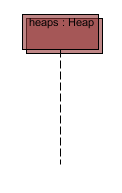
\includegraphics{chap-gedrag/seq-multi-object.png}
%	\centering
%	\caption{Een multi-object}
%	\label{fig:multi-object}
%\end{figure}
%
%\begin{itemize}
%	\item Voor alle leden van een verzameling tegelijkertijd kan een associatie genavigeerd worden. Als op een verzameling S van objecten van klasse X \textit{getY()} wordt uitgevoerd waar Y de naam is van een klasse geassocieerd met X, dan is het resultaat een verzameling van objecten van klasse Y. Die verzameling bestaat uit alle objecten die in verband staan met minstens \'e\'en object uit S.
%	\item $getNumX()$ waar X de naam is van een klasse die in verband staat met de klasse van de verzameling. Het resultaat is de som van het aantal instanties van klasse X waarmee elk lid van de verzameling in verband staat.
%	\item $EXISTS\ ONE\ WHERE\ [query]$: Geeft \textbf{true} als en slechts als \textit{query} geldt voor minstens \'e\'en lid van de verzameling. \textit{query} betekent hier een instructie die bestaat uit getters van klassevariabelen verbonden met booleaanse connectieven (klassevariabelen kunnen hierbij rechtstreeks vergeleken worden met een getal of string, waar toepasselijk).
%	\item $EXISTS\ n\ TO\ m\ WHERE\ [query]$ waar $n \leq m$: Geeft \textbf{true} als en slechts als voor minstens $n$ en ten hoogste $m$ leden van de verzameling geldt dat \textit{query} waar is.
%	\item $FOR\ ALL\ APPLIES\ [query]$: Geeft \textbf{true} als en slechts als voor alle leden van de verzameling \textit{query} geldt.
%	\item $NOT\ [query]$: geeft \textbf{true} als en slechts als \textit{query} \textbf{false} geeft. \textit{query} kan hier \'e\'en van de voorgaande soorten instructies zijn.
%	\item $CHOOSE\ ALL\ WHERE\ APPLIES\ [query]$: Geeft een nieuwe verzameling die bestaat uit alle leden van de originele verzameling waarvoor \textit{query} waar is.
%	\item $CHOOSE\ ONE\ WHERE\ APPLIES\ [query]$: Geeft \'e\'en object uit de verzameling waarvoor \textit{query} waar is. Dit vormt een keuzepunt bij simulatie.
%	\item $CHOOSE\ n\ TO\ m\ WHERE\ APPLIES\ [query]$ waar $n \leq m$: Geeft een nieuwe verzameling die bestaat uit minstens $n$ en ten hoogste $m$ leden uit de originele verzameling waarvoor \textit{query} waar is. Dit vormt een keuzepunt bij simulatie.
%	\item $CHOOSE\ <getalnaam>\ WHERE\ APPLIES\ [query\ dat\ <getalnaam>\ bindt]$: Geeft een nieuwe variabele met als naam \textit{getalnaam} waarvoor geldt dat de waarde voldoet aan \textit{query}. Dit soort instructie kan ook toegepast worden op een variabele dat maar \'e\'en object voorstelt. Dit vormt een keuzepunt bij simulatie.
%	\item $SET <klassevariabele> TO <waarde>$: Voor alle leden van de verzameling wordt de waarde van de genoemde klassevariabele veranderd naar de genoemde waarde.
%\end{itemize}
%
%We illustreren het gebruik van deze nieuwe instructies door middel van het voorbeeld van figuur \ref{fig:new-nim}, dat een modellering van het bekende spel Nim voorstelt. De beurt gaat eerst aan de gekozen speler. Dan wordt gecontroleerd of alle stapels leeg zijn. Als dat niet het geval is, kiest de speler eerst een stapel en neemt dan minstens \'e\'en object weg van die stapel. Daarna wordt de beurt gegeven aan de volgende speler. Als alle stapels leeg zijn, is de huidige speler de winnaar. Dit stelt dus een versie van Nim voor waar de speler die als laatste een object wegneemt verliest.
%
%\begin{figure}[H]
%	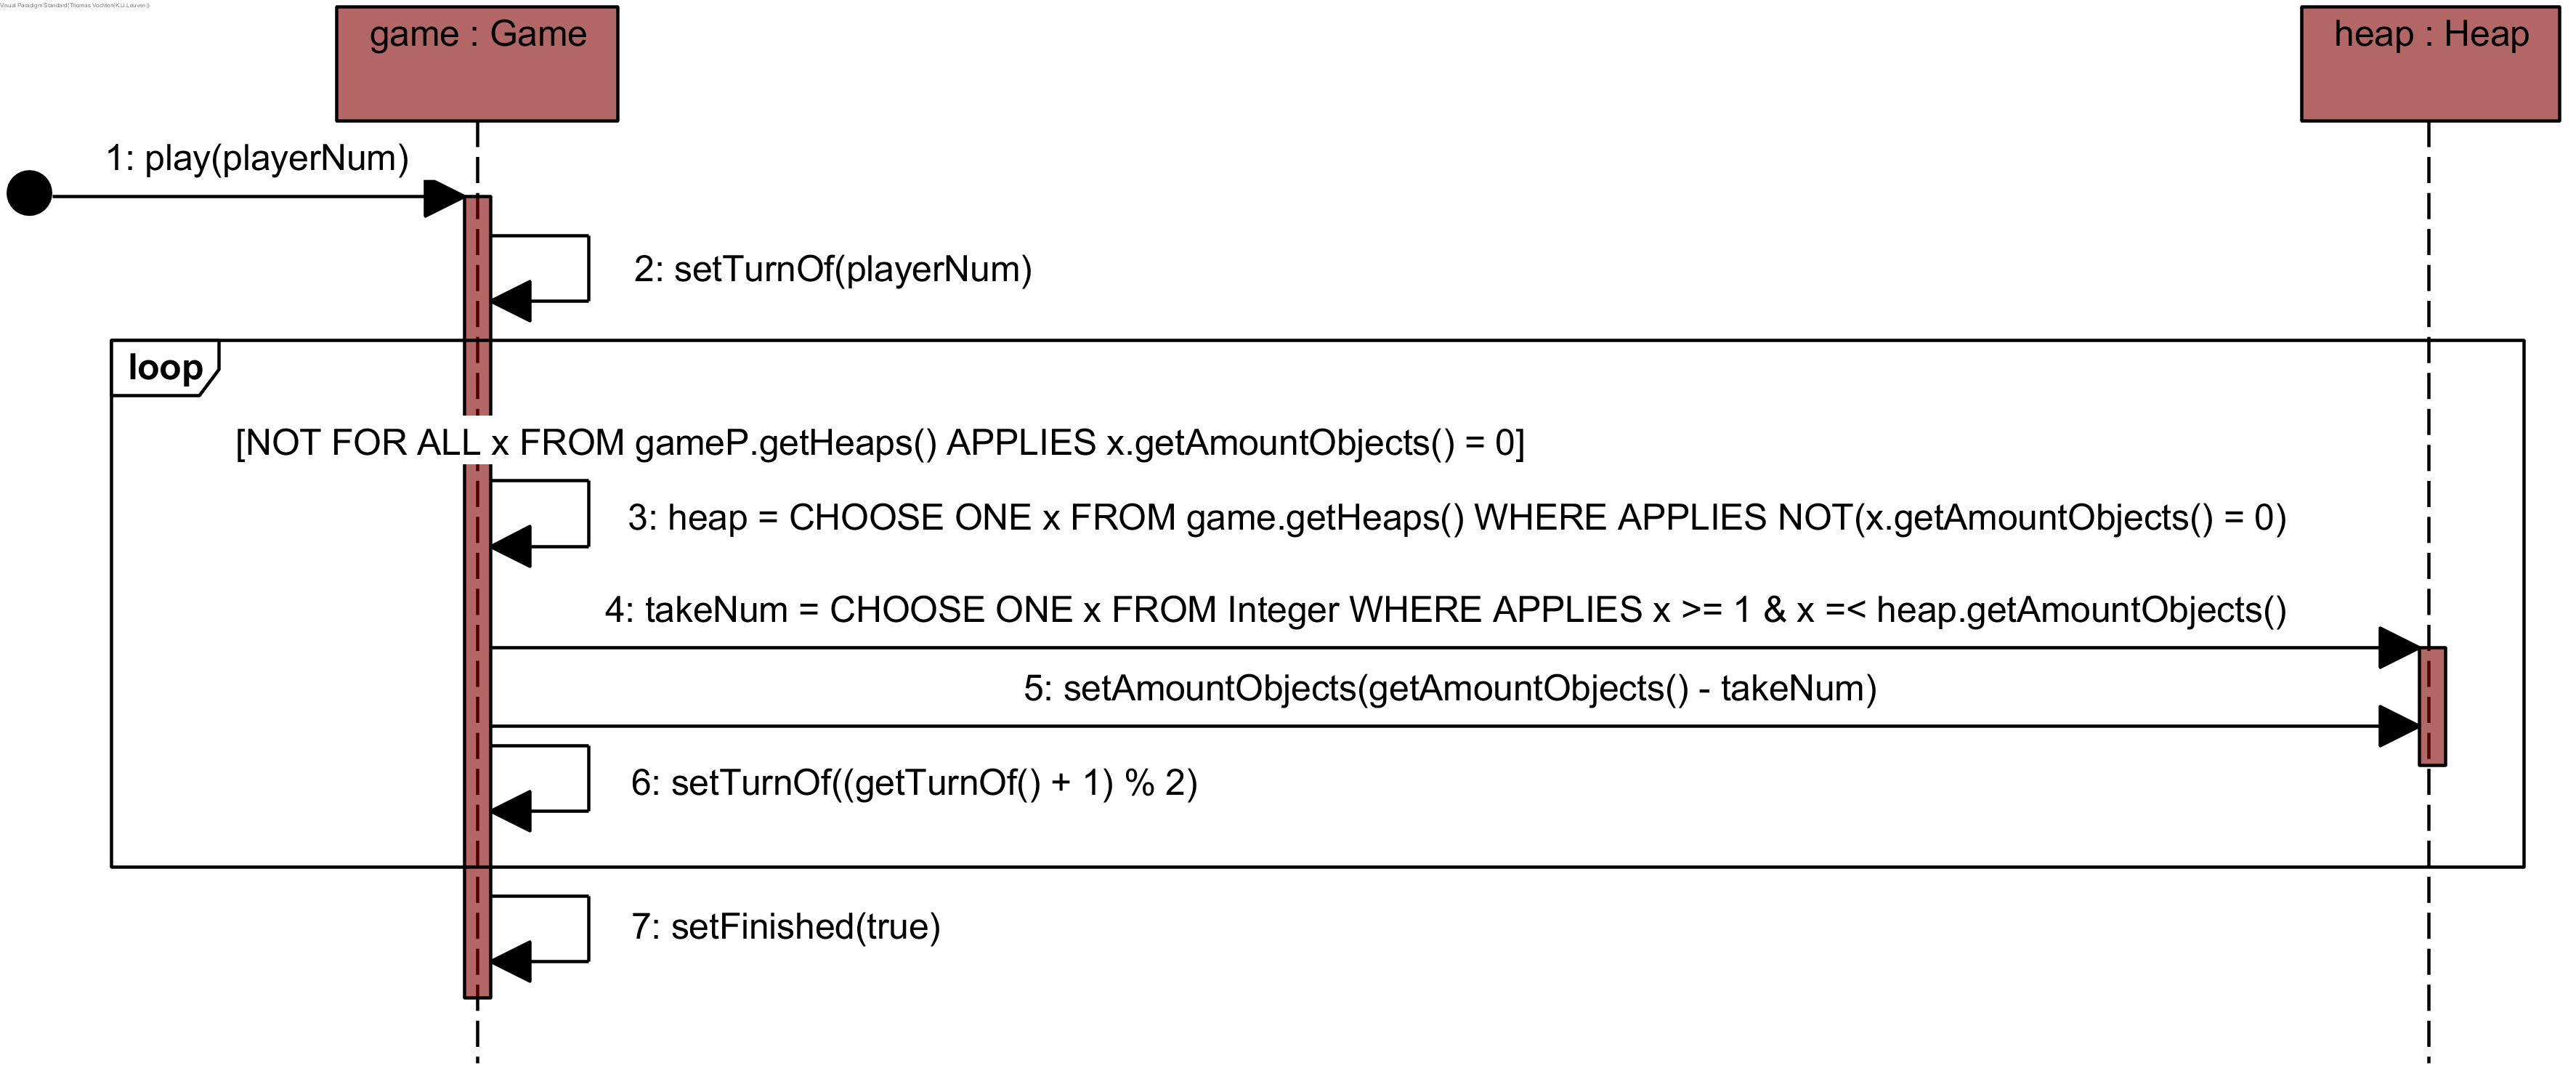
\includegraphics[width=\textwidth]{chap-gedrag/seq-new-nim.png}
%	\caption{Een modellering van het spel Nim}
%	\label{fig:new-nim}
%\end{figure}
%
%De lusvoorwaarde wordt als volgt gebruikt:
%
%\begin{align}
%	\nonumber &\forall{t}[Time]\forall{st}[StackLevel](C\_SDPointAt(Next(t), play\_3) \leftarrow \\ \nonumber &(CurrentStackLevel(t) = st) \land (SDPointAt(t, play\_2) \lor SDPointAt(t, play\_6)) \land \\ \nonumber &\lnot{}\exists{g}[Game](GameT(t, st, g) \land{}\forall{h}[Heap](GameandHeap(g, h) \\ &\Rightarrow \exists{n}[LimitedInt](HeapamountObjects(t, h, n) \land n = 0)))). \\
%	\nonumber &\forall{t}[Time]\forall{st}[StackLevel](C\_SDPointAt(Next(t), play\_7) \leftarrow \\ \nonumber &(CurrentStackLevel(t) = st) \land SDPointAt(t, play\_6) \land \exists{g}[Game](GameT(t, st, g) \land \\ \nonumber &\forall{h}[Heap](GameandHeap(g, h) \\ &\Rightarrow \exists{n}[LimitedInt](HeapamountObjects(t, h, n) \land n = 0)))).
%\end{align}
%
%In instructie 3 wordt de $CHOOSE\ ONE\ WHERE\ APPLIES\ [query]$ instructie gebruikt. We introduceren hier een open predicaat, $ChosenHeap(Time, Heap)$, om ons te helpen deze instructie te vertalen. We voegen de volgende zin toe aan het definitieblok voor diagramvariabelen:
%
%\begin{align}
%	\nonumber &\forall{t}[Time]\forall{st}[StackLevel]\forall{h}[Heap](C\_HeapT(Next(t), st, h) \\ &\leftarrow (CurrentStackLevel(t) = st) \land SDPointAt(t, play\_3) \land ChosenHeap(t, h)).
%\end{align}
%
%Om ervoor te zorgen dat exact \'e\'en Heap-object wordt gekozen, moeten we voorwaardes leggen op $ChosenHeap/2$. Dit doen we als volgt:
%
%\begin{align}
%	&\forall{t}[Time](SDPointAt(t, play\_3) \Rightarrow \exists_{=1}{h}[Heap](ChosenHeap(t, h))).\label{form:uniqueheap} \\
%	\nonumber &\forall{t}[Time]\forall{h}[Heap](ChosenHeap(t, h) \Rightarrow (SDPointAt(t, play\_3) \\ \nonumber &\land \exists{g}[Game]\exists{st}[StackLevel]\exists{n}[LimitedInt]((CurrentStackLevel(t) = st) \\ &\land GameT(t, st, g) \land GameandHeap(g, h) \land HeapamountObjects(t, h, n) \land \lnot(n = 0)))).\label{form:correctsd}
%\end{align}
%
%Zin \ref{form:uniqueheap} garandeert dat er maar \'e\'en \textit{Heap}-object mag gekozen worden.
%
%Zin \ref{form:correctsd} garandeert dat er enkel een keuze mag gemaakt worden als de uitvoering instructie 3 bereikt en dat er enkel een \textit{Heap}-object wordt gekozen waarvoor geldt dat \textit{amountObjects} groter is dan 0.
%
%Voor instructie 4 introduceren we op een soortgelijke manier een open predicaat $ChosenTake/2$. De zin die we toevoegen aan het definitieblok voor variabelen en de voorwaarden die we opleggen op $ChosenTake/2$ zien er gelijkaardig uit.
%
%Bijlage \ref{code:new-nim} bevat de vertaling van het diagram in figuur \ref{fig:new-nim}.